\chapter{LoRa}

LoRa stands for \textbf{Lo}ng \textbf{Ra}nge. It is a transmission standard that aims at achieving long range reach with low power consumption, most commonly used by the Internet of Things devices. LoRa technology was first developed by Cycleo from Grenoble, France around 2010 with first prototypes implementing point-to-point communication for walkie-talkie and metering applications \cite{trinity_panel}. Later in 2012 the Cycleo team was aquired by Semtech, and later released the chips for LoRa end devices and gateways \cite{origins}. \\

The open, non-profit organization LoRa Alliance emerged in 2015 \cite{alliance}. It is an association of companies, with Semtech being one of its founding members \cite{alliance_founder}, backing up the LoRaWAN protocol, ensuring its global presence and acceptance. The total number of alliance members surpassed 500 in 2017 \cite{500_members}. Among the notable members are Cisco, Amazon and Alibaba \cite{alliance_members}. 

\subsection{LoRa Spread Spectrum (Chirp Spread Spectrum)}

% There are 2 main modulation techniques used for radio broadcasting: AM, i.e amplitude modulation and FM, i.e. frequency modulation whereby either amplitude or frequency are modulated. \\

Chird Spread Spectrum is a modulation scheme, whereby the frequency of a signal is changing linearly in time \cite{ieee_2007} as shown on the figure below \ref{fig:slope}. Such sweeps in frequency are called chirps. CSS is a modulation technique that has been around since 1940s
\cite{semtech_spec} with applications in naval and air military and also observed in fauna \cite{origins}.\\

In regards to LoRa CSS signals are bounded by the specified symbol duration and bandwidth. This can be seen in the figure \ref{fig:slope} below. Symbol duration $t_s$ determines the time period over which the frequency sweep occurs and bandwidth defines the sweep range between starting frequency $f_{min}$ and $f_{max}$, i.e. bandwidth = $f_{max} - f_{min}$. Moreover the sweep can start at any frequency $f_0$ (determined by the number of input bits) between $f_{min}$ and $f_{max}$ and this means that a signal can be represented by multiple chirps. So if the sweep reaches $f_{max}$ before $t_s$ it 
continues from $f_{min}$ until time = $t_s$. Thus if $f_0 = f_{min}$
the signal will end at $f_{max}$ exactly without breaking up. 

\begin{figure}[H]
  \centering
  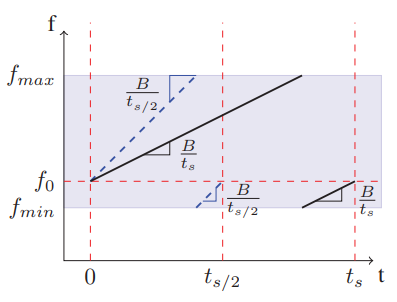
\includegraphics[scale=0.5]{figures/slope.PNG}
  \caption{Graphical representation of the frequency in time for 2 spreading factors. Source: \cite{slope_diagram}}
  \label{fig:slope}
\end{figure}

% What makes CSS different from other Spread Spectrum techniques (despite some claiming it to be a subtype of DSSS \cite{orthogonality_description}) is the fact that it is resistant to multi-path fading and Doppler effect while having relatively moderate transmission power demands \cite{semtech_spec}. \\

% Spreading factor determines the number of bits to be encoded in a signal \cite{sf}

% LoRa employs six spreading factors from 7 to 12 to provide orthogonality in data transmission (collision-free) occurring on the same frequency.  SF determines the chirp rate — change in frequency with respect to time which is the slope on \ref{fig:slope}{}

% An advantage of LoRa spread spectrum is that timing and frequency offsets between transmitter and receiver are equivalent, greatly reducing the complexity of the receiver design. \cite{semtech_spec}  

\subsection{Spreading factors}

According to the Semtech specification \cite{semtech_spec} symbol duration $t_s$ can be calculated using this formula:
\begin{align}
    T_S = \frac{2^{SF}}{B} 
\end{align}

Where $SF$ stands for spreading factor. Thus looking at figure \ref{fig:slope} SF determines the slope of the chirps, i.e. $\frac{B}{T_s}$ and the number of bits in the encoded information \cite{sf_article}, i.e. $f_0$.\\

According to the spec \cite{semtech_spec} LoRa employs 6 spreading factors from 7 to 12. Spreading factors allow different signals to be transmitted over the same channel at the same time. As the specification claims it is possible due to the orthogonality of CSS signals of different spreading factors to each other \cite{semtech_spec}.
Despite the claim, spreading factors have been shown to be quasi-orthogonal and the decoding of signal at the receiver can be disrupted under certain conditions for example if the power of the interfering signal is stronger than the one being decoded \cite{imperfect_1}.

\section{LoRaWAN}

On top of the physical layer there needs to be a protocol. And such is the LoRaWAN layer backed by the LoRa Alliance. As the LoRa Alliance itself states on its website \cite{lora_alliance_about_lorawan} LoRaWAN is a network protocol of communication between Internet of Things devices.

\subsection{Network Topology}

The LoRaWAN standard is based on a star topology.
Multiple end devices (nodes) communicate with a gateway (base station) and multiple gateways communicate with the main network server as demonstrated in the figure \ref{fig:star}. Here gateway acts as an agent between the nodes and the internet, translating Radio Frequency messages into Internet Protocol packets and vice-versa \cite{lora_alliance_about_lorawan}.
One gateway can typically cover a range of hunderds of meters to tens of kilometers with up to millions of end devices \cite{doppler}.

\begin{figure}[h!]
  \centering
  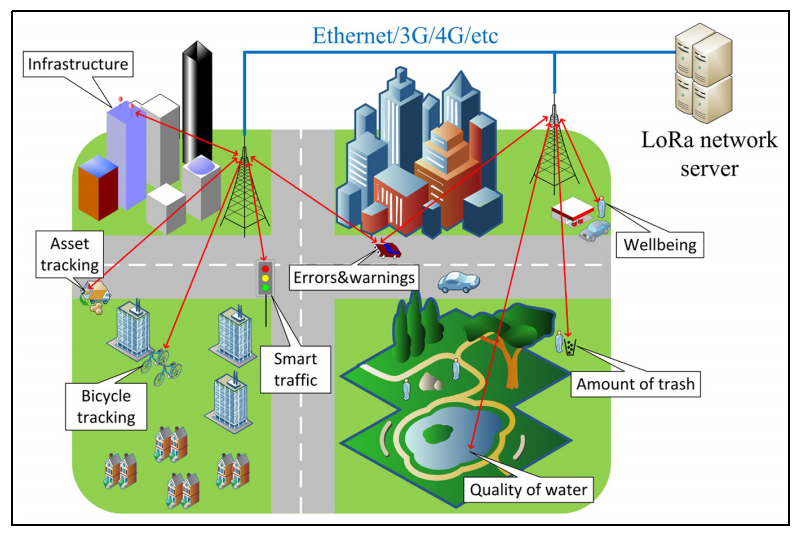
\includegraphics[scale=0.4]{figures/start-topology.PNG}
  \caption{LoRaWAN nodes and gateways connected to a LoRa server Source: \cite{doppler}}
  \label{fig:star}
\end{figure}

\subsection{Multiple Access Control (MAC) scheme}

LoRaWAN implements ALOHA protocol where any device can wake up and transmit a message regardless of time. We are concerned with the messages between a LoRaWAN device and a gateway (base station). Requests from a node to a gateway are called uplink messages, and the responses are called downlink messages.  
The communication scheme has an uplink-centric design and 
LoRaWAN mandates this design for all devices implementing the protocol \cite{simulator}. In the figure \ref{fig:class A} one can see the typical cycle a node goes through while communicating with a particular gateway. The receive windows are allocated periods of time when the node is expecting 
a downlink response that should follow its uplink request.

\begin{figure}[h!]
  \centering
  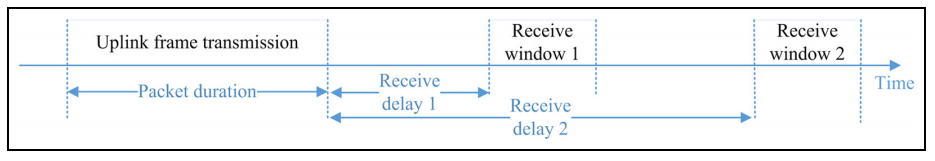
\includegraphics[scale=0.5]{figures/class A.PNG}
  \caption{Class A type LoRaWAN device scheduling of receive slots for downlink messages. Source: \cite{doppler}}
  \label{fig:class A}
\end{figure}

There are 3 different device types based on the way to schedule the receive window slots for downlink communication: class A, B and C. Support for class A (demonstrated in the figure \ref{fig:class A} above) is compulsory with B and C being extensions to it. Class A devices schedule 2 receive windows following an uplink transmission, class B devices open receive windows periodically and class C devices listen for downlink messages continuously unless they are transmitting \cite{lora_alliance_spec}. 

\subsection{Duty cycle}
For each band LoRaWAN devices operate in, they need to comply with the industrial, scientific and medical (ISM) regulations often set by the local government \cite{duty_cycle}. These include the duty cycle limitation that determines amount of time a device can be active within a bandwidth. For example in Europe the duty cycle standards are set by the 
European Telecommunications Standards Institute (ETSI) \cite{about_etsi}.\\
% "the recognized regional standards body dealing with telecommunications, broadcasting and other electronic communications networks and services.", as their website   states.\\ 

What duty cycle basically controls is the fraction of time a device can be active on a particular sub-band (potentially on multiple channels) \cite{duty_cycle}. For example if the channel in 
question is used for 1 time unit for every 10 time units,
the device using it has a duty cycle of 10\%. If we take into account multiple channels (within one sub-band), then we count in the total fraction of time these channels are being used by the device \cite{duty_cycle}.
% [INFO ABOUT section 7.2.3 of the ETSI EN300.220 standard]

\section{NOMA}
 
 Non-Orhogonal Multiple Access (NOMA) scheme is a relatively new concept first introduced in this publication \cite{noma_original} in 2013. As opposed to orthogonal
frequency division multiplexing (OFDM), NOMA decodes multiple incoming signals, occupying the same time 
or frequency resources, utilizing the power or code domain \cite{noma_imperial}. 
% [DIAGRAM FROM TUTORIAL]. 
In the power domain implementation of NOMA the decoding is achieved via successive interference cancellation (SIC) based on the different power levels of the incoming signals \cite{noma_imperial} \cite{noma_original}. \\

Basically what happens is that the incoming signals are decoded at the receiver in the order of decreasing channel gain, so the  strongest one is decoded first and the weakest is decoded last. Signals are decoded in that order so as to minimize the interference different signals experience \cite{noma_imperial}. After the strongest current signal is decoded, the total interference for other signals (to be decoded yet) is reduced by its largest component.\\

Despite the original paper \cite{noma_original} focusing on the downlink NOMA
implementation (i.e. end-device/node being the receiver in question), we are interested in the uplink communications and thus the workings of NOMA at the gateway. 
  
%  As the name NOMA suggests, it it does not utilizes the orthogonality of 
%  , but instead decodes multiple incoming signals based on the 
 
 
\section{LoRa Simulation Framework}

In order to simulate a LoRaWAN network I have decided to pick one described in this paper \cite{simulator}. The developers of the paper have closely followed guidelines from The Things Network (TTN)\footnote{https://www.thethingsnetwork.org/}, which is an open community of volunteers that took on an initiative to contruct and maintain LoRaWAN stations around the world to reach its global coverage. On their website they also provide tutorials and guides to help people deploy LoRaWAN gateways and nodes. The simulation code is published in github \cite{simulator_github}. The developers have decided to simulate the LoRaWAN network via \texttt{SimPy} which is a Python discrete-event simulation framework library\cite{simpy}. The simulation is mainly driven through continuous yielding of appropriate generator functions. 
% A potential improvement to the code would be introduction of some sort of parallelisation.

\subsection{Architecture}

The simulation is based on the LoRaWAN architecture of star-toppology network with mutiple nodes connected to a single gateway as already described above and in the figure \ref{fig:star}. The simulation supports only one gateway, so among other improvements would be introduction of multiple gateways in the simulated area. \\

In the following figure \ref{fig:architecture} is the scheme describing relations between the most relevant simulation python classes (along with their names).

\begin{figure}[h!]
  \centering
  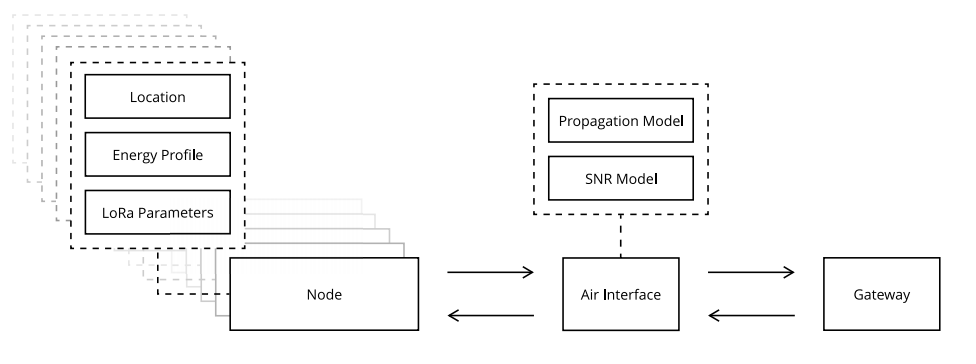
\includegraphics[scale=0.6]{figures/architecture.PNG}
  \caption{Interaction between python classes in the LoRa framework \cite{simulator}}
  \label{fig:architecture}
\end{figure}

\subsection{Nodes}

As can be seen from the figure \ref{fig:architecture} the \texttt{Node} object is characterized by the \texttt{Location}, \texttt{Energy Profile} and \texttt{LoRa Parameters} objects (among others) passed to its constructor during initialization as parameters.\\

\texttt{Location} as its name suggests, simply holds the coordinates for a particular Node. The simulation assumes a rectangular cell, and the particular node location is uniformly at random selected within the bounds of that rectangle. \\

\texttt{Energy Profile} holds information about the different power states and their duration in the execution loop of communication between a node and its respective gateway (sketched above in \ref{fig:class A}). The energy profile used in the original paper \cite{simulator}, as the authors stated was motivated by the energy consumption analysis of another project — LoRaWAN implementation for the EFM32 Happy Gecko develop board \cite{energy_profile}. The energy profile used is displayed in the figure below:

\begin{figure}[H]
  \centering
  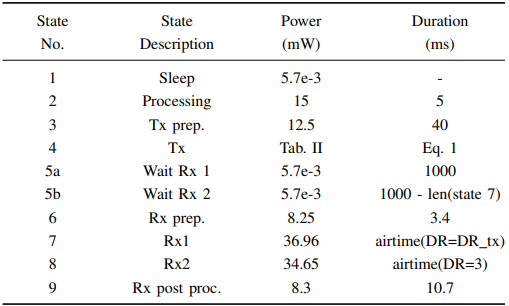
\includegraphics[scale=0.7]{figures/energy_profile.PNG}
  \caption{Energy Profile devised from \cite{energy_profile}. Source: \cite{simulator}}
  \label{fig:energy_profile}
\end{figure}\\

The effect of implementing this energy profile can be seen in the figure \ref{fig:power_states} below; it displays, how the power states of a node develop in time:

\begin{figure}[H]
  \centering
  \hspace*{-1cm}  
  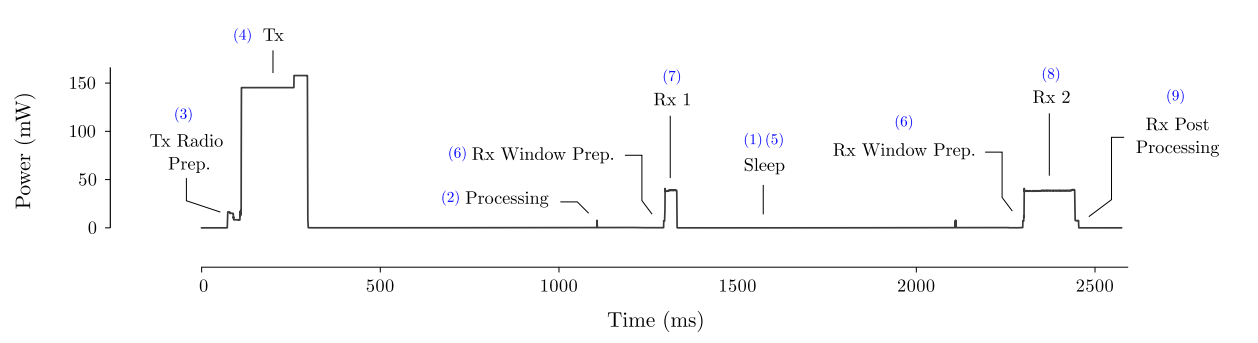
\includegraphics[scale=0.5]{figures/class A 2.PNG}
  \caption{Power states of a LoRa node simulated in \cite{simulator}}
  \label{fig:power_states}
\end{figure}\\

\texttt{LoRa Parameters} object holds information about the configuration of the uplink packets that the Node is going to send, such as its spreading factor, frequency (channel) and transmission power. Subsequently these factors play an immediate role in the resulting energy consumption at the node.
% \cite{simulator}.

\subsection{AirInterface}

\texttt{AirInterface} is the object via which \texttt{Node} and \texttt{Gateway} communicate. It processes the packets "in the air" and determines their airtime as well as simulating collisions between packets. It is also defined by the \texttt{Propagation Model}.
This model is used when determining the received signal
strength of an incoming packet based on its transmission power parameter. \\

\texttt{Propagation Model} calculates the path loss 
of a signal traveling in the channel through the air.
The formula is defined in the original paper \cite{simulator} :
\begin{align}
    PL(d) = PL(d_0) + 10n\times log\frac{d}{d_0} + X_{\sigma} [dB] \label{eq:propagation_model}
\end{align}

Where the following parameters are used. These measurements were taken by the authors \cite{simulator} from measurements reported here \cite{propagation_model_parameters}):
\begin{align*}
     d_0 & = 1000 \text{m}\\
     PL(d_0) & = 128.95 \text{dB}\\
     X_{\sigma} & = 7.8 \text{dB}\\
     n & = 2.32\\
\end{align*}

Collision model is not implemented as a separate object but through a collection of functions in \texttt{Air Interface}. The model implementation is motivated by the authors \cite{simulator} by the findings from another paper \cite{collision_conditions}, that looks at how reception overlap, carrier frequency, spreading factor and power can create conditions for a packet collision. The authors \cite{simulator} also assume that signals with different spreading factors are practically orthogonal and can be demodulated without colliding.\\

% \texttt{SNR} model was implemented in the original framework to
% calculate the Signal-to-Noise ratio values for the packets in the air, but in my implementation I'll use another metric 
% described later in my modifications.

\subsection{Gateway}

\texttt{Gateway} object is responsible for receiving 
the uplink packets from the \texttt{Air Interface}. In order for a packet to come through it must not collide and have  a signal strength above that of gateway's specified sensitivity. On top of that the gateway ensures that the duty cycle restrictions for each channel are satisfied. This is done through
calculating off times, i.e. periods during which the 
channel in question cannot be used. The calculation
involves such \texttt{LoRa Parameters} as frequency,
spreading factor and data rate. The gateway decides 
whether the packet is discarded or the response in 
the form of downlink is required. It also decides on the
receive slots for the response, i.e. $RX1$ or $RX2$.\\

In the original simulator \cite{simulator} \texttt{Gateway} is also responsible for executing the ADR algorithm. ADR is the algorithm, devised to minmize the energy consumption at nodes, operating mainly by estimating the appropriate TP and SF values for each uplink packet and sending them to the respective node (that sent the packet) via a downlink frame \cite{simulator}. The node that uses these values until a next update from the gateway. In the original simulator these values are calculated based on the SNR values of the received frames. \\
% [INPUT DETAILS ON ADR and ADR itself maybe] \\

In this project, however I am not going to implement any form of ADR and instead apply reinforcement learning tecnhiques to 
decide on appropriate \texttt{LoRa Parameters} values for uplink frames.\\

% Due to the SF orthogonality assumption, the gateway can simultaneously receive up to 8 different packets on separate channels. [FALSE???]

\chapter{Reinforcement Learning} 

Reinforcement Learning has recently seen a rise in popularity after a few successful case studies such as the success of DeepMind in 2016 after AlphaGo beat the Korean 9-dan professional Go player \cite{alpha_go_lee_sedol} and after more recently OpenAI beat a team of professionals in a Dota 2 match \cite{dota}.\\

Reinforcement Learning (RL) typically focuses on the problems of agents within some environment. The agents try to learn optimal behaviour within the environment, with the goal of maximizing some sort of reward (e.g. AlphaGo playing Go, trying to maximize it's win probability \cite{alpha_go_lee_sedol}). The policy of that agent, i.e. how it decides to act under certain conditions (e.g. coordinates on a map, temperature, board game position) is the component, not specified by the programmer but instead learnt by the agent via trial-and-error interactions with the environment over the learning period \cite{sutton_barto}. Thus RL often reduces to a problem of learning the optimal policy in the context of a particular application.\\

This closed loop can be demonstrated as in the figure \ref{fig:closed_loop} below, where an agent subject to state $S_{t}$
and reward $R_{t}$ takes an action $A_{t}$ which leads to a new
state $S_{t+1}$ and a new reward $R_{t+1}$:

\begin{figure}[h!]
  \centering
%   \hspace*{-1cm}  
  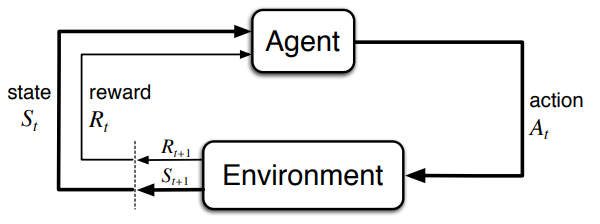
\includegraphics[scale=0.7]{figures/closed_loop.PNG}
  \caption{Closed-loop of reinforcement learning. Source: \cite{sutton_barto}}
  \label{fig:closed_loop}
\end{figure}\\  

% \section{Terminology and symbols}
% Here I'll explain the main bulk of terminology specific to reinforcement learning that we'll need for the rest of this chapter.\\

% Rewards, Action, States, Policy, Value function [DO LATER]
 
\section{Markov Decision Process}

In this section I'll touch upon the basic mathematics of evaluating the environment around the learning agent and the 
main concepts that will be used later in the 
Deep Reinforcement Learning model section.

Markov Decision Process is a Markov Chain based decision making
tool defined by state space $S$, action space $A$, transition 
probability matrix $P^{a}_{ss'}$, reward 
% $P^{a}_{ss'} = p(s_{t+1}| s_t, a_t)$
function $R$ and decision policy $\pi$ \cite{lecture_mdp}. In 
the subsections below I will explain what each of these is.

\subsection{Markov chain}
Markov Chain is essentially a way to model stochastic
processes with particular properties. As the name suggests it is a chain of states that describes the process we are modeling. Using an exmaple from this article \cite{markov_chain_article}, if we
are to model weather at a particular region on a daily basis,
we could have 2 states: Sunny and Rainy. Now what interests us
are the transitions between these 2 states. We could model
them as a simple random process such that the probability of
it being Sunny after being Rainy was 0.5 and the probability
of it being Rainy after being Sunny was 0.1. Furthermore if we
assume the \textbf{memorylessness} property of this model i.e.
that the weather tomorrow is \textbf{independent} of the
weather yesterday and only depends on the weather today then
we could effectively derive the other 2 missing probabilites
for the weather staying Sunny (1 - 0.1 = 0.9) or Rainy (1 -
0.5 = 0.5) for 2 days in a row \cite{markov_chain_article}. This example is demonstrated in figure \ref{fig:weather}.

\begin{figure}[H]
  \centering
%   \hspace*{-1cm}  
  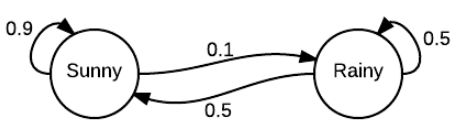
\includegraphics[scale=0.7]{figures/markov_weather.PNG}
  \caption{Markov chain for weather forecasting. Source: \cite{markov_chain_article}}
  \label{fig:weather}
\end{figure}

Thus we can describe a Markov process through a set of states S and a probability transition matrix P satisfying the \textbf{Markov property} (memorylessness) \cite{markov_chain_article}:
\begin{align}
    P_{ss'} = P[S_{t+1} = s' | S_{t} = s]\\
    \sum_{s' \in S} P_{ss'} = 1
\end{align}

\subsection{Policy}
As mentioned above an agent within an environment is capable of taking an action a. The sequence of actions taken under 
various conditions is defined by the agent's policy.
A policy $\pi$ is typically a conditional probability distribution that allows an agent to choose its next action in a defined state at a defined time \cite{lecture_lets_go_markov}:
\begin{align}
    \pi_t(a, s) = P[A_t = a | S_t = s]
\end{align}

\subsection{Reward function}
The reward function $R$ maps transitions between states within a
Markov Decision Process to their respective reward values.
$R_{ss'}^{a}$ is the immediate reward an agent receives if starting from state $s$ it takes an action $a$ and transitions to state $s'$.\\

We can also define the total return value $R_t$ which is the estimated sum of all immediate rewards $r$ starting from time-step t:
\begin{align}
    R_t = r_{t+1} + \gamma r_{t+2} + \gamma ^2 r_{t+3} + ... = \sum^{\infty}_{k=0}\gamma^{k}r_{t+k+1} \label{eq:return}
\end{align}

Where $\gamma$ is the discount factor such that $\gamma \in [0, 1]$ \cite{lecture_lets_go_markov}. The discount factor allows the agent to put different weight on immediate and distant rewards, with smaller $\gamma$ being more concerned with immediate results and larger $\gamma$ looking far into the future. 

% \begin{align}
%     R_{ss'}^{a} = E[r_{t+1} | S_{t} = s, A_{t} = a] \label{eq:return_matrix}
% \end{align}

% This is the reward that the agent leaving state s receives upon transitioning at timestep $t+1$.\\

% [WHY DISCOUNTING IS A GOOD IDEA SLIDE 56 https://materials.doc.ic.ac.uk/view/2021/70028/Course\%20Material/7]
\subsection{State Value Function}
State Value Function $V$ is the estimate of the total return one expects to retrieve starting from a state $s$ at time $t$ in the context of a Markov Decision Process with a policy $\pi$ \cite{lecture_lets_go_markov}. If we expand the expectation term:
% \begin{align}
%      
% \end{align}

% If we now account for an MDP policy $\pi$ and expand the original definition \ref{eq:value_function_def} \cite{lecture_mdp}:
\begin{align}
    V^{\pi}(s) &= \EX_{\pi}[R_{t} | S_t = s]  \label{eq:value_function_definition} \\
    &= \EX[\sum^{\infty}_{k=0} \gamma^k r_{t+k+1} | S_t = s] \nonumber \\
    &= \EX[r_{t+1} + \gamma \sum^{\infty}_{k=0} \gamma^k r_{t+k+2} | S_t = s] \nonumber \\
    &= \EX[r_{t+1} + \gamma R_{t+1} | S_t = s] & \text{definition \ref{eq:return}} \nonumber \\
    &= \EX[r_{t+1} + \gamma \EX[R_{t+1} | S_t = s] | S_t = s] & \text{Adam's Law} \nonumber \\
    &= \EX[r_{t+1} + \gamma V^{\pi}(S_{t+1}) | S_t = s] & \text{definition \ref{eq:value_function_definition}} \nonumber \\
    &= \EX[r_{t+1} + \gamma V^{\pi}(s') | S_t = s] \nonumber \\
    &= \sum_{a \in A} \pi(s, a) \sum_{s' \in S} P^{a}_{ss'} (R^{a}_{ss'} + \gamma V^{\pi}(s')) &\text{expanding $\EX$} \label{eq:mdp_value_function_expansion}
    \label{eq:value_function_def}
\end{align}

where 
\begin{align*}
    \pi(a, s) &= P[a|s] &\text{policy i.e. probability of taking action $a$}\\
    P^{a}_{ss'} &= P[s' | s, a] &\text{state-action transition probability}\\
    R^{a}_{ss'} &= r(s, a, s') &\text{immediate reward function}
\end{align*}

% Converting the last line of the above derivation into vector notation to account for n states (respectively n dimensions):
% \begin{align}
%     \textbf{v} = R + \gamma P \textbf{v}
% \end{align}

% A direct solution to this would be 
% \begin{align}
%     \textbf{v} = (\bbone - \gamma P)^{-1}R
% \end{align}

% Due to matrix inversion being an expensive computational operation, this kind of approach of estimating a state value function is not preferred and only works for relatively small MRPs \cite{lecture_lets_go_markov}. There are, however iterative approaches to this problem, such as Dynamic Programming, Monte-Carlo evaluation and Temporal Difference Learning.\\

Majority of all the reinforcement learning algorithms introduced in this chapter later down below will rely on this "recursive consistency" \cite{lecture_mdp} property of state value functions. 

% \subsection{Policy Evaluation}
% Now we need to find a systematic way of estimating the value
% function for a given MDP for an arbitrary policy. This process is called Policy Evaluation \cite{lecture_mdp}. The most obvious method is to apply the Bellman equation over and over again, until the value function converges as in figure \ref{fig:ipa}.
% \begin{figure}[H]
%   \centering
% %   \hspace*{-1cm}  
%   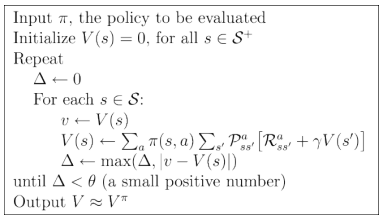
\includegraphics[scale=0.8]{figures/iterative_policy_evaluation.PNG}
%   \caption{Iterative Policy Algorithm; Source: \cite{lecture_mdp}}
%   \label{fig:ipa}
% \end{figure}

\subsection{State Action Value Function}
As an extension to the state value function we introduce the state-action value function $Q$ that evaluates the expected return for taking action $a$ at a state $s$ subject to policy $\pi$ \cite{lecture_mdp} :
\begin{align}
    Q^{\pi}(s, a) = \EX[R_t | S_t = s, A_t = a] = \EX[\sum^{\infty}_{k=0} \gamma^k r_{t+k+1} | S_t = s, A_t = a]
\end{align}

The relationship between state value and state-action value functions is as follows:
\begin{align}
    V^{\pi}(s) = \sum_{a \in A} \pi(s, a) Q^{\pi}(s, a) 
\end{align}

% An important advantage of the state-action value function over state value function is the 

\section{Learning Approaches}

In this section I'll look at different learning approaches such
as Dynamic Programming and Monte-Carlo methods and how 
these rely on agent's Model Knowledge. The final Deep Reinforcement Learning model will be based of each of these 
and will heavily rely on concepts introduced here as well. 

\subsection{Policy Improvement}

The term "learning" implies that the agent iteratively attempts 
to find a better policy than the current one it is using. 
Through the Policy Improvement Theorem \cite{lecture_dp} it is 
possible to compare 2 policies against each other and determine
which one is better based on the State Value or State-Action
Value functions it induces. Based on that it is possible to run a
Policy Iteration Algorithm \cite{lecture_dp} which iterates
through all states of an MDP and different policies are evaluated and then improved on using the equation \ref{eq:value_function_def} derived earlier.

\subsection{Dynamic Programming}

Dynamic Programming typically refers to a set of algorithms targeted at solving problems within well-defined systems such as Markov Decision Process \cite{lecture_dp}. Typically Dynamic Programming refers to solving a problem by breaking it into smaller sub-problems and solving them recursively. This kind
approach can be taken with the MDP defined above in regards to 
the recursive equation \ref{eq:value_function_def}. It is an
example of "bootstrapping" where the value function
for a current state is calculated from the value function 
estimations for neighbouring states \cite{lecture_dp}. \\

DP works well for moderate not resource hungry type of problems and suffers from the curse of dimensionality once the problem complexity increases. It also requires full knowledge of the Markov Decision Process which is not always available in practice. Hence the next subsection. 

\subsection{Monte Carlo (MC) Methods}

Monte-Carlo Methods are fundamentally different from the 
Dynamic Programming approach in that they don't require the 
full knowledge of the environment around the agent. They fall
in the category of Model-free learning algorithms \cite{lecture_mfl}. The process is based fully on the sampled experience.  \\

The basic idea is to calculate the average return over traces of episodes, an episode being state transition of the type sampled directly from the environment. A state transition ($S, A, R, S'$) includes information about original state $S$, chosen action $A$, immediate reward $R$ and the resulting state $S'$. One condition is that each episode trace must end in a terminal state $S_{terminal}$. 

\subsubsection{Monte-Carlo update rule}

Like in the Policy Improvement subsection one can devise the policy evaluation algorithm based of calculating the average return over traces of episodes \cite{lecture_mfl}. 
% Here you can see that value function is approximated with an average returns of states. This is a First-Visit MC algorithm, so only the first occurence of a state is counted toward the estimate. In Every-visit MC algorithm every occurence is recorded \cite{lecture_mfl}.
% We can update the policy after every episode or after
% sampling a trace of 20 for example. the former is called online MC and the latter Batch MC.
To update the mean value for a state after each transition an incremental update from the normal definition of 'mean' can be devised as described here \cite{lecture_mfl} :
\begin{align}
    \mu_k &= \frac{1}{k}\sum^{k}_{i = 1} x_i \nonumber \\
    &... \nonumber \\
    \mu_k &= \mu_{k - 1} + \frac{1}{k} (x_k - \mu_{k - 1})
\end{align}

This is an important milestone, since the running mean can be recorded without storing traces of transitions. In the same way one can update the state value function $V(s)$ (as in Monte-Carlo it holds the average reward over episodes of experience) incrementally after each new episode (s, a, r, s'):
\begin{align}
    V(s_t) \longleftarrow V(s_t) + \frac{1}{N(s_t)}(R_t - V(s_t))
\end{align}

Moreover one can set the $N(s_t)$ value (i.e. current number of sampled transitions) to another number $n$, such that $n < N(s_t)$, by basically narrowing down the averaging operation to the last n transitions. This is in effect turns the fraction into $\alpha$ -- the rate at which old episodes are discarded \cite{lecture_mfl}:
\begin{align}
    V(s_t) \longleftarrow V(s_t) + \alpha (R_t - V(s_t)) \label{eq:mc_increment}
\end{align}

\subsection{Temporal Difference}
% We have now introduced two different approaches to finding the optimal Value function for a problem at hand: Dynamic Programming and Monte-Carlo. Dynamic programming achieves the optimal solution through "bootstrapping" i.e. estimating state values through
% neighbouring states. Monte-Carlo methods calculate the estimates through sampling directly from experience i.e. traces of episodes. \\

Temporal Difference (TD) is what combines Dynamic Programming and Monte-Carlo: like MC It does not require full model knowledge of Markov Decision Process at hand and 
learns from episodes of experience and like DP it makes use of bootstrapping \cite{lecture_mfl}.

% \begin{figure}[h!]
%   \centering
% %   \hspace*{-1cm}  
%   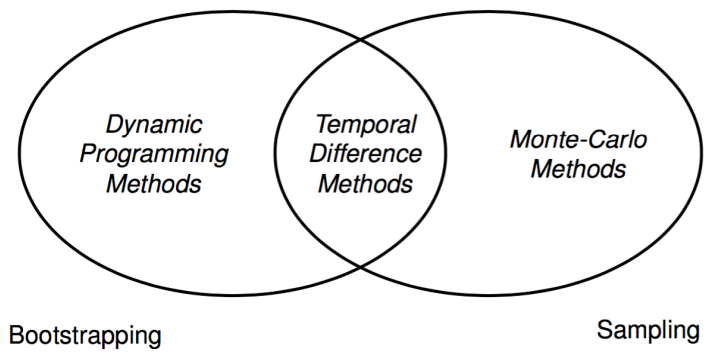
\includegraphics[scale=0.5]{figures/TD_diagrams.PNG}
%   \caption{Temporal Difference; Source: \cite{lecture_mfl}}
%   \label{fig:td}
% \end{figure}

The combination of DP and MC is manifested in the value function update rule for Temporal Difference:
\begin{align}
  V(s_t) \longleftarrow V(s_t) + \alpha (r_{t+1} + \gamma V(s_{t+1}) - V(s_t)) \label{eq:td_update}
\end{align}

where:
\begin{align*}
  r_{t+1} + \gamma V(s_{t+1}) - V(s_t) &\text{ — } \text{TD error}\\
  r_{t+1} + \gamma V(s_{t+1}) &\text { — } \text{TD target}
\end{align*}

Comparing this to the update rule for MC (equation \ref{eq:mc_increment}) we can see that in addition to the actual measured reward $r_{t+1} (R_{t}$ in equation \ref{eq:mc_increment}) we add an estimate of the next state i.e. $V(s_{t+1})$. This estimation refers us back to the original estimation of the value function from equation \ref{eq:value_function_def} making TD target an estimation of the total expected return.\\

Thus in the Temporal Difference Value estimation algorithm
bootstrapping and direct sampling are combined \cite{lecture_mfl}. 

% \subsection{Bias-Variance tradeoff for TD and MC}
% In statistics the Bias-Variance tradeoff typically refers to 
% a compelled compromise between variance and bias, i.e. either high variance and low bias or low variance and high bias. \\

% We can see that $R_t = r_{t+1} + \gamma r_{t+2} + \gamma ^2 r_{t+3} + ...$ is an unbiased estimate of $V^{\pi} (s_t)$ by the definition \ref{eq:value_function_def} of the state value function itself. So if the update rule for TD was $r_{t+1} + \gamma V^{\pi}(s_{t+1})$ it would be an unbiased estimate of $V^{\pi}(s_{t})$ (given $V^{\pi}(s_{t+1})$ is the true value function). But what we actually have is an estimate of the $V^{\pi}(s_{t+1})$ — $V$ ($r_{t+1} + \gamma V(s_{t+1})$ in the update rule) and so the expression for TD target is the biased estimate of $V^{\pi}(s_t)$ \cite{lecture_mfl}. \\

% Now if we compare TD and MC methods we can see that TD has some bias with MC being generally unbiased, at the same time TD has much lower variance since the estimate is based only on one transition (s, a, r, s'), while MC return estimate depends on many transitions (trace of episodes). The immediate implications of this is that MC methods have good convergence,
% if the simulation runs for long enough but TD is usually more efficient, so it requres less time to learn the value function \cite{lecture_mfl}.

% But due to its nature it is more sensitive to the initalization values for value function.

\section{Model Free Control }
In this section I'll focus on the two well known 
Temporal Difference algorithms approaching the model-free
setting from 2 perspectives. 

% We cannot refer to MDP in 2 scenarios: MDP is simply unknown or MDP is well defined but too big to generalise/estimate (Curse of dimensionality).

\subsection{From V to Q} 
First it needs to be said that applying Policy Iteration that is typically used in DP or MC contexts is not feasible here, since the Policy Improvement Theorem is based on the State Value Function estimation through Bellman's equation \cite{lecture_mfc}, as mentioned above. This is what the policy update step would look like for such iteration algorithm (remember equation \ref{eq:value_function_def})
\begin{align}
    \pi(s) \leftarrow arg \max_{a} \sum_{s'} P^{a}_{ss'} [R^{a}_{ss'} + \gamma V(s')]
\end{align}

Here the state transition probability matrix $P$ and 
the immediate reward function $R$ require model-knowledge
which puts it outside of the model-free paradigm \cite{lecture_mfc}. One solution is to replace $V$ with 
State-Action Value function $Q$, which fits the 
model-free narrative better, since no model knowledge
is required, only Q function is involved:  
\begin{align}
    \pi(s) \leftarrow arg \max_{a} Q(s, a) 
\end{align}

\subsection{On and Off policies}
There are 2 different approaches to using policies for 
generating training data and evaluating the model: on-policy and
off-policy methods.
% One of the important prerequisites for the above proof is the 
% «Exploring starts» assumption, 
% i.e. the agent needs to learn the optimal policy by infinitely selecting all possible actions. There are 2 ways to ensure the agent continues to 
% explore all options: on-policy and off-policy methods. \\
\textbf{On-policy} methods use one policy to estimate value functions and choose actions (i.e. generate data), while \textbf{off-policy} methods separate these into 2 policies \cite{lecture_mfc}. 

\subsection{Soft control}

Soft policies have a property such that all actions have a chance to be explored, i.e. $\pi(a, s) > 0$ $\forall s \in S, \forall a \in A.$\\

A form of soft-policies are $\epsilon-$greedy policies, where 
you can adjust a parameter $\epsilon$ to weigh a particular action such that it has a higher probability of being chosen,
while all the other actions are equally probable (relative to each other) \cite{lecture_mfc}:\\\\
$\epsilon$-greedy policy with $\epsilon \in [0, 1]$:
\begin{align}
    \pi(s, a) = \begin{cases} 
        1 - \epsilon + \frac{\epsilon}{|A(s)|}, \text{ if } a^{*} = arg \max_{a} Q(s, a) \\
        \frac{\epsilon}{|A(s)|}, \text{ if }  a \neq a^*
    \end{cases}   
\end{align}

An important convergence condition is "Greedy in the
Limit with Infinite Exploration" \cite{lecture_mfc} 
(GLIE). It specifies that in order for the learning model
to converge, $\epsilon$ needs to be reduced over time 
so that the $\lim_{k \to \infty} \epsilon_{k} = 0$ with $\epsilon_{k} = \frac{1}{k}$ for instance.

% \subsection{batch learning}

% Like before there are 2 MC approaches: batch learning and online learning

% \begin{figure}[h!]
%   \centering
% %   \hspace*{-1cm}  
%   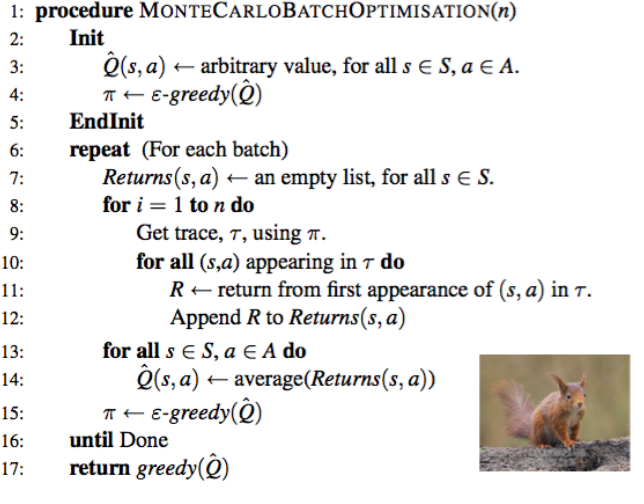
\includegraphics[scale=0.5]{figures/mc_batch_greedy.PNG}
%   \caption{MC Batch Learning to Control; Source: Lecture}
%   \label{fig:mc_batch_greedy}
% \end{figure}
% \begin{figure}[h!]
%   \centering
% %   \hspace*{-1cm}  
%   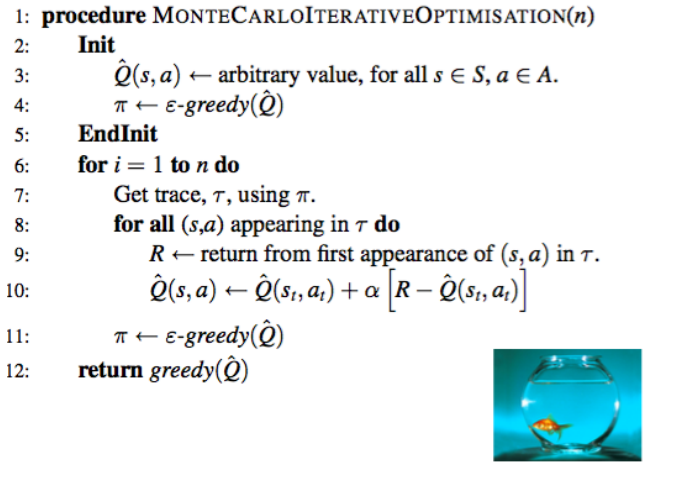
\includegraphics[scale=0.5]{figures/mc_iterative_greedy.PNG}
%   \caption{MC Iterative Learning to Control; Source: Lecture}
%   \label{fig:mc_iterative_greedy}
% \end{figure}

% \subsection{MC summary}
% one of the issues in MC is sufficient exploration of all available actions. In simulated environments this issues can be tackled with randomness for state-action values at the start of  the learning process but harder to arrange in learning from real experience. \\

% "In on-policy the agent commits to exploration and learns the respective stochastic policy while in off-policy an agent learns a deterministic policy separate from the one followed. Typically off-policy methods rely on some form of importance sampling."

\subsection{Temporal Difference Control -- SARSA}
Temporal Difference has several advantages over MC such as lower variance and online learning so we can combine the $\epsilon$-greedy policy improvement and TD update rule from equation \ref{eq:td_update} with Q(S,A) \cite{lecture_mfc} (basically replacing V with Q) :
\begin{align}
    Q(S, A) \longleftarrow Q(S, A) + \alpha (r + \gamma Q(S', A') - Q(S, A)) \label{eq:sarsa_update_rule}
\end{align}
% \begin{figure}[h!]
%   \centering
% %   \hspace*{-1cm}  
%   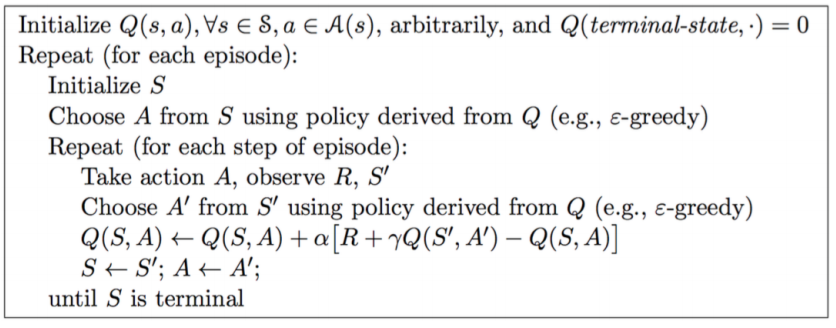
\includegraphics[scale=0.5]{figures/sarsa.PNG}
%   \caption{SARSA - On-Policy learning TD control; Source: \cite{lecture_mfc}}
%   \label{fig:sarsa}
% \end{figure}

This update rule forms the SARSA algorithm, deriving its name
from the typical transition an agent undergoes -- 
($S$, $A$, $R$, $S^'$, $A^'$)\\

\begin{algorithm}[H]
\SetAlgoLined
Arbitrarily initialize $Q(s, a), \forall s \in S, \forall a \in A$\;
initialize S arbitrarily\;
from S choose action A using the $\epsilon$-greedy policy $\pi$\;
\While {$S$ is not $S_{terminal}$}{
take action A, observe R, S^{'}\; \\
from $S^{'}$ choose action $A^'$ using the $\epsilon$-greedy policy $\pi$ \;
Q(S, A) \longleftarrow Q(S, A) + \alpha (R + \gamma Q(S', A') - Q(S, A))\;\\
S \longleftarrow S^{'}\;\\
A \longleftarrow A^{'}\;\\
}
\caption{SARSA -- on-policy temporal difference learning. Source: \cite{lecture_mfc} }
\label{algorithm:sarsa}
\end{algorithm}\\

On top of the GLIE convergence condition SARSA also needs
to satisfy the Robbins-Monroe sequence of learning rates $\alpha$: 
\begin{align*}
    \sum^{\infty}_{t=1} \alpha_{t} &= \infty \\
    \sum^{\infty}_{t=1} \alpha_{t}^{2} & < \infty \\
\end{align*}

So something like $\alpha_{k} = \frac{1}{2^{k}}$ will 
work \cite{lecture_mfc}.

% "One issue for SARSA is sparse rewards when the reward 
% propagates down a trace through many episodes slowly. Two ways to deal with it are SARSA-Lambda and Hindsight Experience Replay"

\subsection{Off-policy Q-learning}

As mentioned above in off-policy a different policy  $\pi'$ is used to generate the data while estimating and optimizing $Q^{\pi}$ and $V^{\pi}$ still. $\pi$ is the target policy and $\pi'$ is the  behaviour policy. An important assumption to ensure learning the assumption of coverage: $\pi(a, s) > 0 => \pi'(s, a) > 0$ \cite{lecture_mfc}.\\

% "One of the most important breakthroughs in reinforcement learning was the development of off-policy TD control algorithm known as Q-learning (Watkins, 1989)." [LECTURE]

In Q-learning the  next action is chosen using the behaviour policy, but in the update rule we use the alternative greedy successive action based on the target policy: $\max_a Q(s_{t+1}, a)$\\

In this way both the target and behaviour policies improve, target policy being greedy w.r.t. $Q(S, A)$ and behaviour policy being $\epsilon$-greedy w.r.t $Q(S, A)$. The Q learning target is then respectively: $r_{t+1} + \max_{a'} \gamma Q(s_{t+1}, a')$\\

% \begin{figure}[h!]
%   \centering
% %   \hspace*{-1cm}  
%   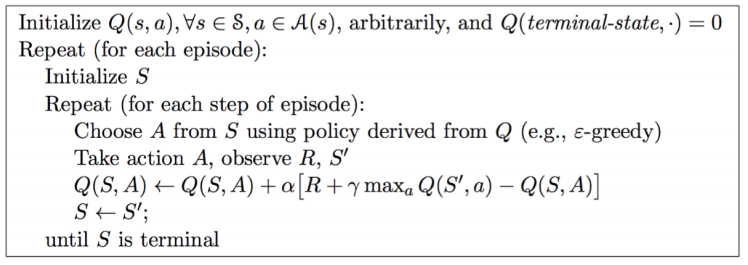
\includegraphics[scale=0.5]{figures/q_learning.PNG}
%   \caption{Q-Learning algorithm; Source: \cite{lecture_mfc}}
%   \label{fig:q_learning}
% \end{figure}

\begin{algorithm}[H]
\SetAlgoLined
Arbitrarily initialize $Q(s, a), \forall s \in S, \forall a \in A$\;
initialize S arbitrarily\;
\While {$S$ is not $S_{terminal}$}{
from S choose action A using the $\epsilon$-greedy behaviour policy $\pi'$\;
take action A, observe R, S^{'}\; \\
Update Q function using the greedy target policy $\pi$, i.e. $\max_{a}$ term\; 
Q(S, A) \longleftarrow Q(S, A) + \alpha (R + \gamma \max_{a} Q(S', a) - Q(S, A))\;\\
S \longleftarrow S^{'}\;\\
}
\caption{Q-learning -- off-policy temporal difference learning. Source: \cite{lecture_mfc} }
\end{algorithm}\\


There are no explicit policies here: target policy is implicit in the greedy term $max_a Q(S', a)$ and behaviour policy is the $\epsilon$-greedy version of the target policy that we use to choose $A$. Both policies are updated with the update rule.

\subsection{Cliff walking  Q-learning vs. SARSA}
One very well known example demonstrating the difference between
Q-learning and SARSA or in other words Off-policy and On-policy learning methods was presented by Sutton and Barto \cite{sutton_barto}. They look at a case of an agent traversing a grid from left to right bypassing a cliff's edge as shown in the figure \ref{fig:cliff}. Each
step in the grid gives a reward of -1 and "falling off" 
the cliff results in a reward of -100 and the agent goes
back to the starting position.

\begin{figure}[H]
\centering
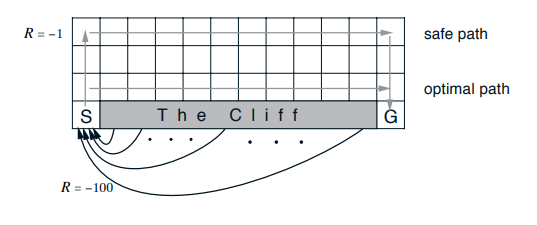
\includegraphics[scale=0.6]{figures/cliff_scheme.PNG}
  \caption{Cliff walking example; Source: \cite{sutton_barto}}
  \label{fig:cliff}
\end{figure}

Here Q-learning and SARSA produce different optimal policies. Q-learning gives the "optimal path" walking near the edge, while SARSA suggests a "safer path" further
from the cliffs edge and despite the former clearly 
being the preferred option, Q-learning still performs 
worse than SARSA based on the overall reward score as can be seen from figure \ref{fig:cliff_score}

\begin{figure}[H]
\centering
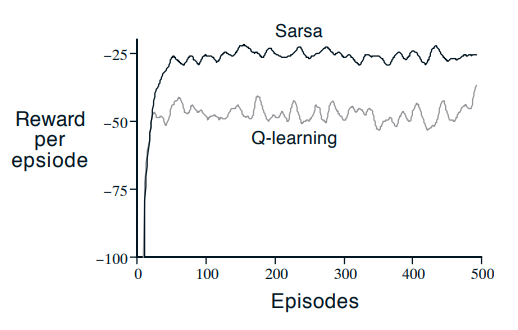
\includegraphics[scale=0.6]{figures/cliff_score.PNG}
  \caption{Cliff walking results; Source: \cite{sutton_barto}}
  \label{fig:cliff_score}
\end{figure}

As Sutton and Barto recognize \cite{sutton_barto} this 
arises precisely from the on and off policy nature of 
these 2 approaches. Q-learning still acts based on its
\textbf{behaviour policy} unrelated to the optimal target policy it optimizes and thus due to it being $\epsilon$-greedy when walking near the cliff it occasionally "falls off" and this affects the overall
reward score.  At the same time because SARSA is 
optimizing the same policy it follows it learns a safer
path further from the edge because it takes the \textbf{next} action selection into account. 
It follows the next selected action as can be seen from the 
algorithm \ref{algorithm:sarsa} and accounts for its Q value.

\section{Function Approximation}

\subsection{Limitations of tabular}

In Tabular Q learning due to the discrete nature of 
state and action spaces it is harder to represent the real world accurately as the problem of fine discretisation arises: the approximation needs to be accurate enough for meaningful learning. But this can be memory inefficient as the number of parameters grows \cite{lecture_intro_to_deep_rl}. \\

Another important limitation affects the exploration ability of the learning agent: each Q entry for subsequent state-action entries need to be updated independently despite obvious correlation between them.\\

One solution to this is function approximation. 

\section{Neural Network}

A neural network consists of multiple layers of interconnected neurons each defined by a weight and bias that are applied to the incoming signal \cite{lecture_intro_to_deep_rl}.\\

In supervised learning there's usually a reference that 
the network is trained against, for example in classification the reference might be a label to an RGB image. The model then learns weights such that the desired outputs are produced on respective inputs \cite{lecture_intro_to_deep_rl} . \\

This is achieved through backpropagation and gradient
descent where the difference between current weights and
desired weights is evaluated using a cost function and
applied until the model converges to a desired state
\cite{lecture_intro_to_deep_rl} .\\

For example for a dataset with $x_i$ input paired with a $y_i$ label cost function would be: 
\begin{align}
    C(\theta, D) = [y_i - f(x_i)]^2
\end{align}

\section{Deep Q learning}

It is possible to approximate the Q-table with a neural network that accepts state and outputs Q(s, a) 
values for the whole range of actions \cite{lecture_intro_to_deep_rl}. For example like in 
figure \ref{fig:q_network} state space can become continuous, while action space is still discrete.

\begin{figure}[H]
  \centering
%   \hspace*{-1cm}  
  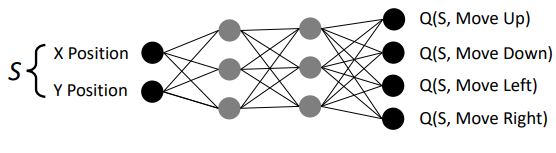
\includegraphics[scale=0.5]{figures/q_network.PNG}
  \caption{Example Q network for traversing a 2D space; Source: \cite{lecture_intro_to_deep_rl}}
  \label{fig:q_network}
\end{figure}

To design a cost function for such a neural network 
one can take the temporal difference error from the update tule \ref{eq:td_update} as the basis \cite{lecture_intro_to_deep_rl}:
\begin{align}
    C(\theta, D) = [R + \gamma \max_a Q(S', a) - Q(S, A)]^2
\end{align}
% \begin{figure}[h!]
%   \centering
% %   \hspace*{-1cm}  
%   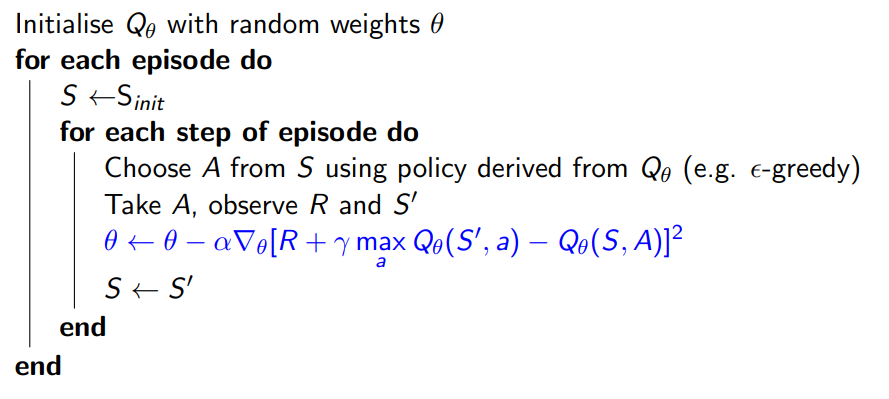
\includegraphics[scale=0.5]{figures/dqn_first.PNG}
%   \caption{Deep Q-learning algorithm; Source: \cite{lecture_dqn}}
%   \label{fig:dqn_first}
% \end{figure}

\begin{algorithm}[H]
\SetAlgoLined
Initialize $Q_{\theta}$ with random weights \theta \; \\
initialize S arbitrarily\;\\
\While {$S$ is not $S_{terminal}$}{
from S choose action A using the $\epsilon$-greedy policy\;
take action A, observe R, S^{'}\; \\
\theta \longleftarrow \theta - \alpha \nabla_{\theta}[R + \gamma \max_{a} Q_{\theta}(S', a) - Q(S, A)]^{2}\;\\
S \longleftarrow S^{'}\;\\
}
\caption{Deep Q-learning. Source: \cite{lecture_dqn} }
\end{algorithm}\\

\subsection{Overfitting}

Overfitting is a common problem of machine learning 
model training in the context of supervised learning.
A potential pitfall is that after training the model
might be tuned too much towards the training data
and will not generalise on previously unseen data well.
To tackle this issue various techniques were introduced, 
e.g. early stopping. \\

In the Reinforcement Learning domain, however the 
overfitting issue cannot arise in the same sense as in
supervised setting, since the agent is constantly 
seeing new data and there is no training period where
the "right" actions are well defined and compared against
as in image classification for example.

% Like any neural network it can overfit but the random starts nature of LR counteracts that in effect [QnA]

\section{Experience Replay Buffer}

One limitation of online learning is that one transition needs to be visited many times for the network to learn appropriate weights ("many updates per transition" \cite{lecture_dqn}). \\

A solution is to create a dataset of all the experienced data so far collected by the agent. The advantage is that any transition can be sampled from the replay buffer and trained on more than once \cite{lecture_dqn}. 

\subsection{Mini batch learning }

Another limitation of deep Q-learning is that since now Q is represented not by a table, but by a continous function, neighbouring state values will affect each other easily due to correlation between them \cite{lecture_dqn} . If the function is updated in a consecutive manner (going by consecutive states in the order they were collected for example) this will cause the Q-distribution to start changing rapidly and affect the untrained parts of the Q-network and cause uneven learning. \\

One solution is to sample transitions from the replay buffer not in the order they were collected but in random mini-batches. This causes a more uniform, even learning and update of the Q function.  

% \begin{figure}[H]
%   \centering
% %   \hspace*{-1cm}  
%   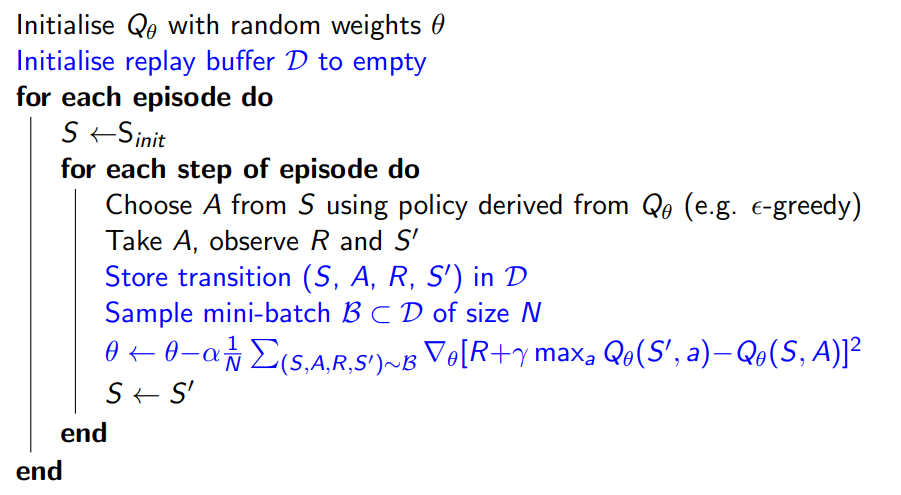
\includegraphics[scale=0.5]{figures/replay_buffer.PNG}
%   \caption{Deep Q -learning algorithm with replay buffer; Source:\cite{lecture_dqn}}
%   \label{fig:replay_buffer}
% \end{figure}

\subsection{Prioritised Experience Replay}

On top of sampling transitions in minibatches in a uniform random manner it may be useful to note that some transitions might be more important than others and sampling them more frequently may boost the learning process. \cite{lecture_dqn}. Hence the idea of prioritised experience replay buffer. \\

A way to tell which transitions are more important than others is to see the magnitude of the prediction error $\delta = R + \gamma \max_a Q_{\theta}(S', a) - Q_{\theta}(S, A)$. 
Intuitively greater error results in greater learning.\\

So each transition is assigned a weight $w_i = |\delta| + \epsilon$, where $\epsilon$ is a small constant ensuring each transition has a probability of being sampled greater than 0. Thus the sampling probability for a transition $i$ is:
\begin{align}
    p_i = \frac{w_i^{\alpha}}{\sum_k w^{\alpha}_k}
\end{align}

Where $\alpha$ determines how much individual transitions are prioritized over the others with $\alpha = 0$ being equivalent to uniform sampling.\\

It only makes sense to update only the weights for transitions that were sampled, since their $\delta$ error values\cite{lecture_dqn} are already known. Newly 
submitted transitions are assigned the current maximum weight to ensure that they can be sampled and that sufficient exploration is done.

% \begin{figure}[H]
%   \centering
% %   \hspace*{-1cm}  
%   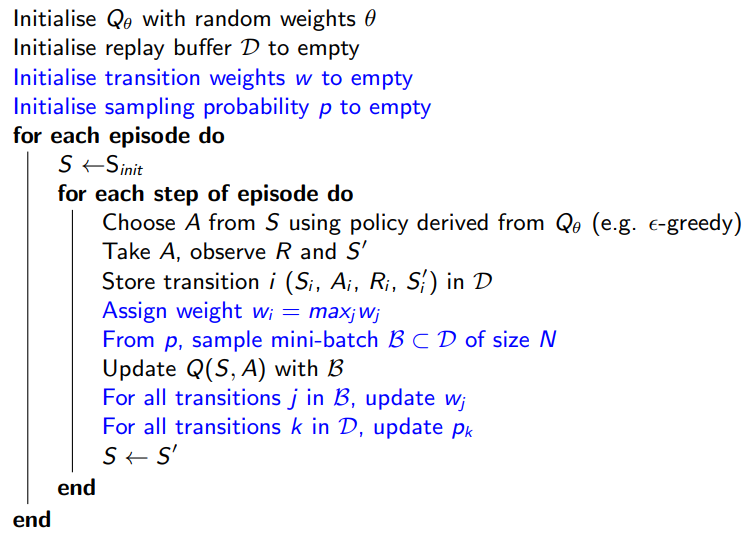
\includegraphics[scale=0.5]{figures/prioritized_buffer.PNG}
%   \caption{Prioritised Experience Replay Algorithm; Source: \cite{lecture_dqn}}
%   \label{fig:replay_buffer}
% \end{figure}

\section{Target Network }

Another problem introduced by generalisation is when adjacent states are trained on multiple times
it results in a rocketing effect \cite{lecture_dqn}.  

\begin{figure}[H]
\centering
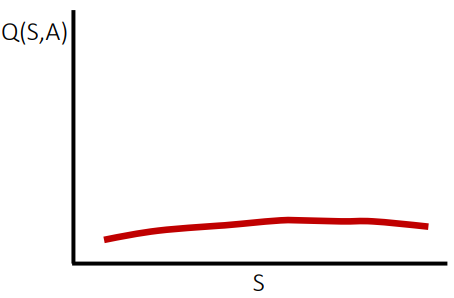
\includegraphics[scale=0.5]{figures/target 1.PNG}
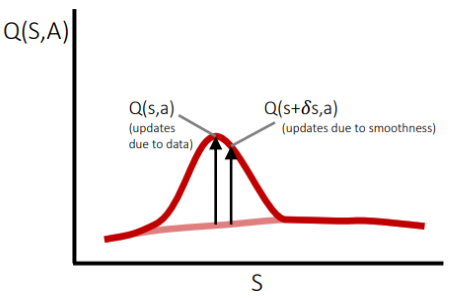
\includegraphics[scale=0.5]{figures/target 2.PNG}\\
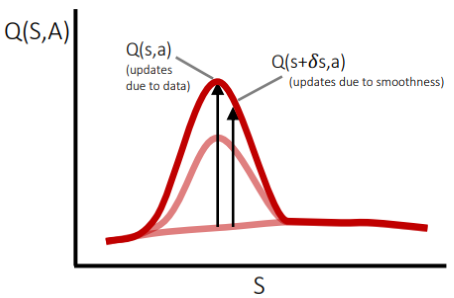
\includegraphics[scale=0.5]{figures/target 3.PNG}
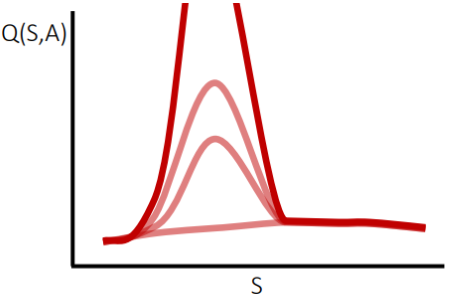
\includegraphics[scale=0.5]{figures/target 4.PNG}
  \caption{Generalisation effect on learning; Source: \cite{lecture_dqn}}
  \label{fig:generalisation_curse}
\end{figure}

This correlation between adjacent states can be tracked down to the $\max_a Q_{\theta}(S', a)$ term in the update step. Hence the 
extension to DQN is to introduce a separate Target Network $\hat{Q}$ to calculate the prediction error. This allows Q network to learn independently from the generalisation effect \cite{lecture_dqn}. Every now and then $\hat{Q}$ is set to Q.

\begin{figure}[H]
\centering
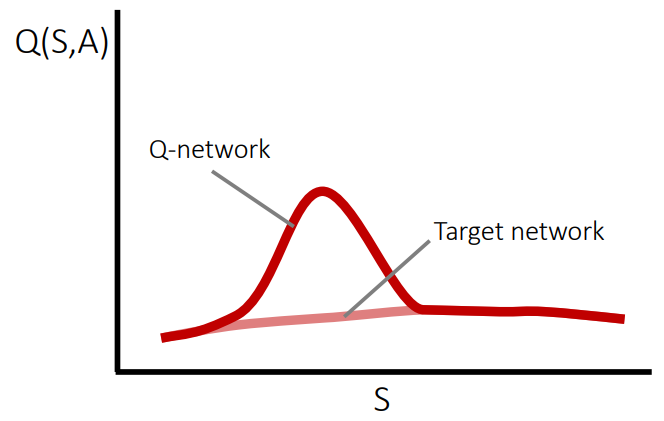
\includegraphics[scale=0.4]{figures/target 0.PNG}
  \caption{Target network; Source: \cite{lecture_dqn}}
  \label{fig:target_network}
\end{figure}

% Here's the updated algorithm for Deep Q-learning with target network extension.

% \begin{figure}[H]
% \centering
% 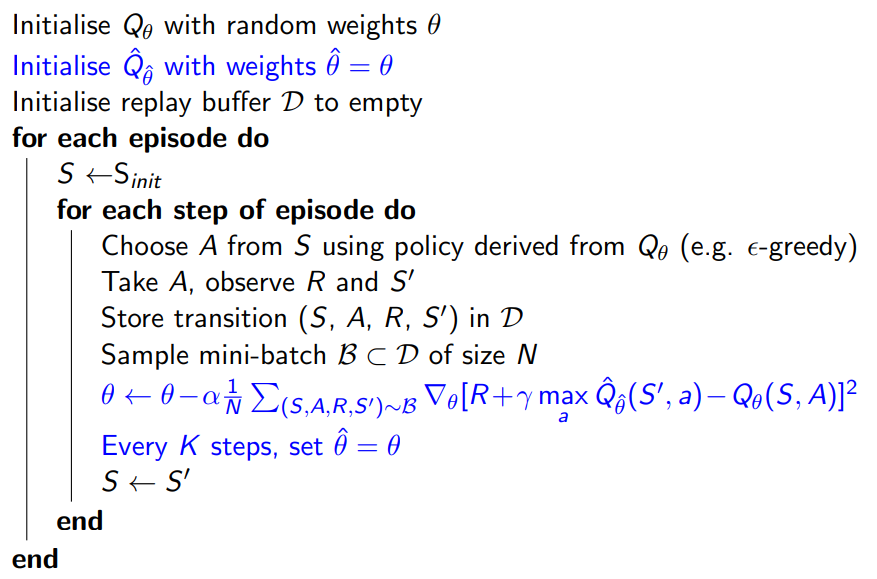
\includegraphics[scale=0.4]{figures/dqn wth target.PNG}
% % \caption{The Universe}
%   \caption{Deep Q-Learning with Target Network; Source: Lecture}
%   \label{fig:target_network_algorithm}
% \end{figure}

\section{Double Deep Q-learning}
Another issue that still arises is the problem of overestimation when picking the greedy action in the target $R + \gamma \max_a \hat{Q}_{\hat{\theta}}(S' a)$. Target network is a noisy estimation for different action values (for an arbitraty state) and the sampled maximum $\hat{Q}$ value might not be the maximum for the true $Q$ function for the same action \cite{lecture_dqn}. In order to tackle this problem of overestimation 
further decoupling is introduced in the target term.\\

In Double Deep Q-learning different networks are used to pick the maximum action and estimate its Q value. This on average reduces the amount by which an action is overestimated since an unusually high value in one network is unlikely to be such in the other \cite{lecture_dqn}. Thus the new error in the update step in the algorithm is either:
\begin{align}
    [R + \gamma Q_{\theta}(S', \text{arg}\max_a\ \hat{Q}_{\hat{\theta}}(S', a)) - Q_{\theta}(S, A)]^2
\end{align}
or:
\begin{align}
    [R + \gamma \hat{Q}_{\hat{\theta}}(S', \text{arg}\max_a\ Q_{\theta}(S', a)) - Q_{\theta}(S, A)]^2
\end{align}

\begin{algorithm}[H]
\SetAlgoLined
Initialize $Q_{\theta}$ with random weights \theta \; \\
Initialize $\hat{Q}_{\hat{\theta}}$ with weights \theta \; \\
Initialize replay buffer $B$\; \\
initialize S arbitrarily\;\\
\While {$S$ is not $S_{terminal}$}{
from S choose action A using the $\epsilon$-greedy policy\;
take action $A$, observe $R$, $S^{'}$\; \\
store transition ($S$, $A$, $R$, $S^{'}$) in B\; \\
sample min-batch D $\subset$ B of size N\; \\
\theta \longleftarrow \theta - \alpha \frac{1}{N} $\sum_{(S,A,R,S^{'}) \sim B} \nabla_{\theta}[R + \gamma Q_{\theta}(S', \text{arg}\max_a\ \hat{Q}_{\hat{\theta}}(S', a)) - Q_{\theta}(S, A)]^{2}$\;\\
Every K steps, $\hat{\theta} = \theta$ \;\\
S \longleftarrow S^{'}\;\\
}
\caption{Double Deep Q-learning with Prioritised Replay Buffer. Source: \cite{lecture_dqn} }
\end{algorithm}\\



% \subsection{3 network architectures}
% \subsection{REINFORCE ALGORITHM}
% \subsection{deterministic vs stsochastic policies}
% \subsection{reducing variance}
% \subsection{model free vs model based}
% \subsection{planning in discrete spaces (irrelevant to LoRa) }
% \subsection{Cross Entropy }
% \subsection{method for continuous spaces (relevant?)}
% \subsection{model predictive control}

\chapter{Learning Model}



\section{Related work in the field}

There have a been a few attempts at implementing resource optimization with Reinforcement Learning. For example the
authors of this paper \cite{rl_lora_original} applied 
Deep Q learning to resource optimization for LoRaWAN
networks and produced promising results for energy
consumption but not for throughput. Their approach
however is the most relatable in terms of the learning
model used. In this paper \cite{rl_lora_sarsa_dqn} both
SARSA and DQN approaches are applied, former used for
light traffic and the latter for heavy traffic, due state
space growing based on the current number of users. On
top of that the actions in that paper mean swapping users
in and out of different channels. The researchers here 
\cite{rl_distributed_mab} took distributed learning
approach with the naive tabular multi-agent multi-arm
bandit (MAB) implementation.

There have apparently been no such studies for NOMA LoRa 
networks and this will be my contribution. 

\section{Learning Model}

In case of ADR optimization the gateway executes the algorithm
and returns the desired parameters to the node via a downlink 
message. Here, however I've decided to implement the learning 
agent on the node side, unlike for example in this paper 
\cite{rl_lora_sarsa_dqn} where the agent is abstracted over the
nodes. In my implementation however each of the nodes
contributes to the learning process and takes a portion of the
agency role upon itself. It contributes to the learning process
both tabular and deep through the data it individually collects.

\section{Distributed Learning and Clustering}
The ideal situation would of course be having one learning agent
per LoRa node so they could learn a policy specifically suited for that one node. But the case is that typically nodes located 
near each other can benefit from one policy as the authors of this paper \cite{rl_lora_original} recognized. However 
in that paper nodes a grouped together based on their 
distance from the node and so clusters are of a circular 
form. 
% [CITATION or EXPERIMENT] 
I wanted to try and make clusters even more local based and divided the simulation cell into 
square sectors of adjustable size as shown in the figure 
\ref{fig:my_sectors} below.

\begin{figure}[H]
\centering
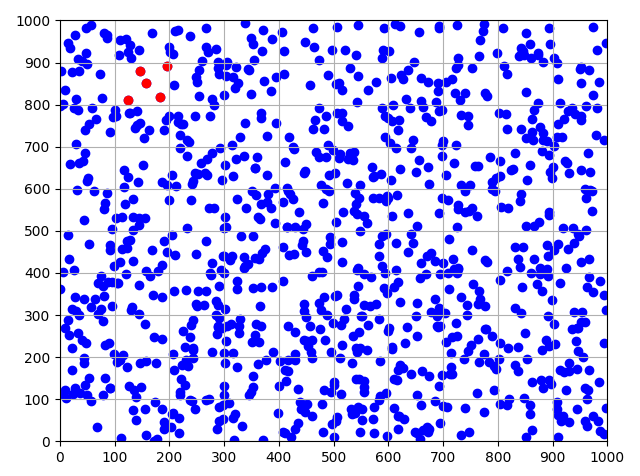
\includegraphics[scale=0.7]{figures/my_sectors.PNG}
  \caption{Grouping of nodes together with one cluster highlighted with red. \\ Sector size = 100 meters}
  \label{fig:my_sectors}
\end{figure}

So in order not to waste memory on slightly different models for nodes located near each other nodes can be grouped into clusters and share Q function (or learning weights
in case of a deep model). \\

Below is the diagram demonstrating the distribution of 
deep learning agents over 3 node clusters.\\

\begin{tikzpicture}
  [node distance=.8cm,
  start chain=going above,]
  
    \node[punktchain, join] (agent2) {Learning Agent 2\\ DQN $\theta_2$};
    
    \begin{scope}[start branch=right0]
    \node[punktchain, on chain=going right] (agent3) {Learning Agent 3\\ DQN $\theta_3$};
    \end{scope}
    
    \begin{scope}[start branch=left0]
    \node[punktchain, on chain=going left] (agent1) {Learning Agent 1\\ DQN $\theta_1$};
    \end{scope}
    
      \node (asym) [punktchain, join] (cluster2) {Node Cluster 2};
      
      \begin{scope}[start branch=left1,
        every join/.style={->, thick, shorten <=1pt}, ]
        \node[punktchain, on chain=going left]
            (cluster1) {Node Cluster 1};
      \end{scope}
      
      \begin{scope}[start branch=right1,]
      \node (cluster3) [punktchain, on chain=going right] {Node Cluster 3};
    \end{scope}
      
  \node[punktchain, join,] (air)    {\texttt{Air Interface}};
  \node[punktchain, join,] (noma)   {\texttt{NOMA}};
  \node[punktchain, join] (gateway) {\texttt{Gateway}};
  
  \draw[|-,-|,-, thick,] (cluster3.north) |-+(0,1em)-| (air.south);
  \draw[|-,-|,-, thick,] (cluster1.north) |-+(0,1em)-| (air.south);
  \draw [|-,-|,->, thick,] (agent1.north) -- (cluster1.south);
  \draw [|-,-|,->, thick,] (agent2.north) -- (cluster2.south);
  \draw [|-,-|,->, thick,] (agent3.north) -- (cluster3.south);

\end{tikzpicture}



\subsection{Reward}

Follwing the introduction of NOMA it makes sense to base
the reward function to a respective metric such as SINR.
Such metric is throughput $T$, which can be calculated as follows: 
\begin{align}
T = log_2(\text{SINR}+ 1)
\end{align}

Furthermore in order to minimize energy consumed at nodes I 
include the reciprocal of energy consumed per bit $E_{bit}$ to the reward
value. So as a result we get:
\begin{align}
    reward = \frac{T}{E_{bit}}
\end{align}

\subsubsection{Reward collection}

One of the main differences between a classical reinforcement
learning model and the LoRa simulator in question is the immediateness of the reward, since in the LoRa simulation the immediate actions don't have an immediate effect on the environment and instead are delayed. The question then arises how to determine that delay and collect the rewards at the right time. \\

As described above each node goes through a cycle (implemented 
as a while loop in the simulation). It constantly repeats
a simple set of actions: sleep, send uplink transmission, sleep,
receive downlink transmission or confirm that the uplink 
packet didn't reach the base station. So naturally I decided to establish this flow:
select and take an action then send the uplink packet,
confirm the state of the downlink transmission, compute
the reward and learn from it. There are other potential 
ways to establish the needed delay, maybe 
establish more wait time but this implementation is the 
simplest one. As in case of a successful uplink transmission
the action taken at the beginning should have a direct effect on the throughput and energy values of that packet 
which should've manifested themselves by the time the receive
windows for the downlink packets are opened. 

\subsection{Action space}
Following the example of this paper \cite{rl_lora_original} the action space consists naturally of the \texttt{LoRaPacket} 
parameters available to Node, i.e. spreading factor,
transmission power and channel (frequency): 
\texttt{[sf, tp, channel]}. \\

A further suggestion would be to explore other parameters from \texttt{LoRaParameters}.

\subsection{State space}
In this simulation I've made the state space adjustable 
so it is possible to run the state space consisting of any 
combination of these parameters (inferred from
\cite{rl_lora_original}): spreading factor (SF), 
transmission power (TP), channel (frequency), received signal
strength (RSS), signal-to-interference-plus-noise ratio (SINR),
energy consumed per bit, packet ID and number of packets:\\
\texttt{[sf, tp, channel, rss, sinr, energy, packet\_id, num\_packet]}

\subsection{Slow Action Traversal}
During hypertuning I experimented with different state spaces
and noticed that between many there's no difference in 
performance, the model seems to output similar results
despite the state space. One of the possible causes for this
is the extensibility of the action space. \\

Unlike in classical RL problems where an agent's action causes
a minor transition in the state space, here for example if 
the state space is \texttt{[sf, channel, tp]} then the agent can just travel from an arbitrary to state to any other point
in the state space, because that's how the action space 
traversal is defined. \\

So I decided to introduce a slower version of action space,
where in each dimension only an incremental update is possible, e.g. from \texttt{sf}7 an agent can only go to \texttt{sf}8 or \texttt{sf}9.

% Despite first prototypes starting with 

% \section{LoRa State}
% \section{LoRa Action}
% \section{LoRa Reward}

\chapter{Modifications to code}

\section{SimPy simulation framework}

\section{Original framework legitimacy}
As mentioned above the simulator code was described in this 
paper \cite{simulator}. The authors presented some plots against
which I could compare. This is the most obvious immediate 
comparison one can make to legitimize this framework and it's
authors claims. Here are the plots from the original paper:

\begin{figure}[h]
\centering
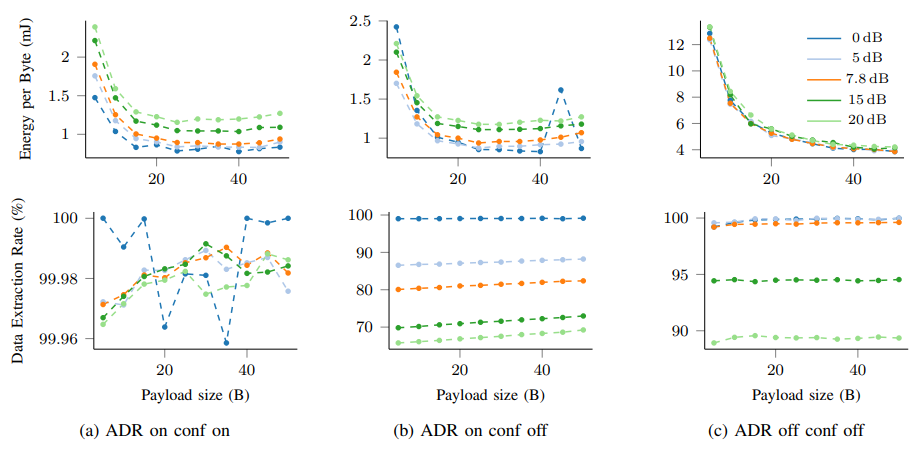
\includegraphics[scale=0.6]{figures/original_plots.PNG}
  \caption{Plots from the original simulator framework paper \cite{simulator}}
  \label{fig:my_sectors}
\end{figure}

And here are my plots for equivalent parameter settings, though
some numerical values had to be inferred:

\begin{figure}[H]
\centering
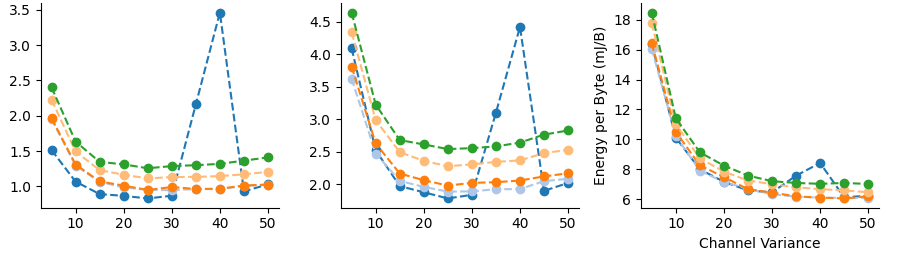
\includegraphics[scale=0.5]{figures/my_plots_1.PNG}\\
\hspace*{1.3cm}  
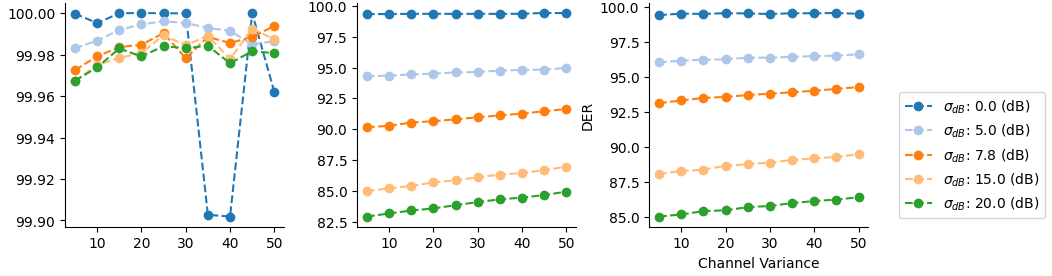
\includegraphics[scale=0.5]{figures/my_plots_2.PNG}
  \caption{Plots generated locally}
  \label{fig:my_sectors}
\end{figure}

Generally the plots seem to follow same trends and portray 
similar values except for a couple of anomalies in the
recordings the values produced by running the simulation
seem to resemble the original paper and the paper along with
the code is trusted and legitimized to that extent. 

\section{NOMA}
The main simulation aspect that enabling NOMA affects is the 
order in which incoming uplink packets are processed by 
gateway. \\

For that matter a \texttt{NOMA} object is introduced. It is 
launched in a way similarly to nodes. It executes a loop
until the end of the simulation time and periodically checks
for packets in the air that have not collided. If there are any
it then picks the one with the strongest received signal 
strength for the gateway to decode. \texttt{AirInterface} keeps
track of packets in the air with a list sorted by the signal
strength for convenience. 

\subsubsection{SINR}
The \texttt{SINR Model} is implemented similarly to how \texttt{SNR Model} was implemented in the original simulator \cite{simulator}. The model calculates signal-to-interference noise ratio (SINR) for the received signal strength values of packets in the air according to this formula:
% [CITE WIKIPEDIA???]:
\begin{align}
    \text{SINR}(x) = \frac{P}{I + N} \label{eq:sinr}
\end{align}
where:
\begin{align*}
     P &- \text{power of the examined signal}\\
     I &- \text{total interference from weaker signals in the air}\\
     N &- \text{ noise floor}\\
\end{align*}

The interference is only calculated from the weaker signals, since we're assuming that NOMA is enabled at 
the gateway and thus all the stronger signals would be
decoded apriori \cite{noma_original}.\\

\texttt{SINR Model} also calculates throughput from SINR values using the formula defined above.
% \subsection{Clustering implementation}

\section{Learning Models}

For most of the project I have focused on Temporal Difference
style learning involving evaluating and improving the Q
function. I have had a go at both naive tabular implementation
mapping State-Action pairs to expected returns and the 
function appoximation of Q with a neural network. 
In particular I have compared side by side Q-learning and SARSA
as their implementation is very similar to each other. \\

Due to its simplicity a Monte-Carlo style update is also 
attempted.
 
\subsection{Learning Agent Interface}
Two learning agents are implemented for Tabular and Deep Q approximation. Despite that they follow the same interface
which allows to switch between them seamlessly so the Node
doesn't need to explicitly know whether he is assigned a 
tabular agent or a deep agent. The interface is as follows:
\texttt{choose\_next\_action} and \texttt{train}. The former 
follows the $\epslion$-greedy policy and chooses the next 
action accordingly as described above. The latter accepts
a transition from nodes assigned to it and updates the Q table
or the neural network accordingly. For the deep implementation
the network is trained on the temporal difference error squared
as described above. \\

\subsubsection{Node taking partial agency}

The node is directly involved in the learning process. 
It calculates its current state and reward for itself thus
producing  unique transition traces which the agent learns from. 
What it does fetch from outside is the next action it should
take. It gets it from the agent and all nodes within a cluster
are fetching actions from one agent, but for each of them
the result will depend on their unique state.\\

In this way the agent benefits from all the nodes assigned to 
it as they all contribute to learning, be it a naive tabular or
deep implementation.

\subsection{Tabular Q}
Tabular Q function is implemented as a \texttt{pytorch} 
tensor mapping the state space \texttt{tp, sf, channel} to 
a list of Q values for all possible actions, each associated
with the index in that list for convenience. Action space 
is subject to hypertuning as well with slow action traversal
available for each action parameter \texttt{sf, tp} or 
\texttt{channel}. For each the slow action space simply 
reduces to \texttt{[-1, 0, +1]} where +1 and -1 means traversing 
the next largest or smallest value in the defined \texttt{LoRa.Parameters} range, for example, given 
\texttt{TRANSMISSION\_POWERS = [2, 5, 8, 11, 14]} if the current 
\texttt{tp} value is 8, then +1 action will result in \texttt{tp} = 11 and -1, repsectively, in \texttt{tp} = 5. In this way 
the agent is closer to a robot walking in a maze and resembles classic reinforcement learning problem setting.

\subsection{Deep Q}
Deep Q network maps state space to action space in the same way
as tabular does, the difference being adjustability of the state
space as this only affects the input dimensions of the network.
So various other values such as SINR and RSS can be added to the 
state space. This is precisely why the latter is preferred 
as it allows for flexibility in implementation and as we'll 
see later it converges much faster. \\

There are various other way to approximate $Q$ through neural
networks allowing for continuous action spaces as well.
But since the \texttt{LoRa Parameters}, used for constructing
the action space I have, are discrete that is not necessary
in this scenario/setting.\\

Deep Q is represented by a \texttt{Module} class, which is 
the building class for neural networks in \texttt{pytorch}.
The neural network is formed by an adjustable number of 
pairs of Linear Layers and ReLU activation functions.
Thus depth of the model becomes another subject of 
hypertuning. \\



\subsubsection{Neural Network}

For the purposes of training a neural network \texttt{pytorch}
Python library is used. It provides extensive functionality
for machine learning and various additional optimizations.
For this problem I am using a combination of linear layers
paired with ReLU activation functions. \\

There are other well known deep architectures for neural
network models such Convolutional Neural Networks or 
Recurrent Neural Networks. For our input and output 
a linear model suffices and fitting it to CNN and RNN
type input would not make sense or be feasible?


\subsection{Model Convergence}
Two conditions that in theory ensure convergence of the 
learning model are epsilon and alpha decay according to 
GLIE and Robbin-Monroe respectively. As mentioned above.
The plots do seem to suggest significant improvement for the
reward function after they are put in place.\\

PLOT\_HERE

\subsection{Mitigating Generalisation}
\subsubsection{Double Deep Q-learning with Target Network}
\texttt{target\_network} is initialized as an exact copy of the 
\texttt{q\_network} and is used during training to pick the next 
optimal action as described in the background section. 
\texttt{target\_network} weights are synchronized with the
weights of \texttt{q\_network} every 10 steps as defined by the 
\texttt{target\_update\_rate}. Subject to hypertuning?

\subsubsection{Prioritised Replay Buffer}
\texttt{Replay Buffer} is a separate object keeping a buffer
of transitions of size 50 and respectively weights for each one 
of those transitions. Each time a new transition is submitted
it is assigned the maximum current weight. Transitions are 
sampled in batches of 10. They are picked based on the 
probability distribution derived from their respective weights
as described in the background section. As weights are derived 
from the loss each transition induces all weights for 
transitions that were just trained on are updated regularly. 

\section{Neural Network Normalization}
\subsection{Weight normalization}



\subsection{Batch normalization}

\chapter{Hypertuning and Performance}
% Comparison to other models and implementations

\section{GLIE and Robbins-Monroe convergence}
Satisfying the convergence properties for both $\epsilon$
and $\alpha$ is crucial for learning as can be seen from
these plots. \\


Here's a plot of effects of alpha and epsilon decay on tabular Q-learning. As we can see from the rewards plot introducing alpha decay with epsilon decay gives us the best result.
\begin{figure}[H]
\centering
\hspace*{-1.1cm}  
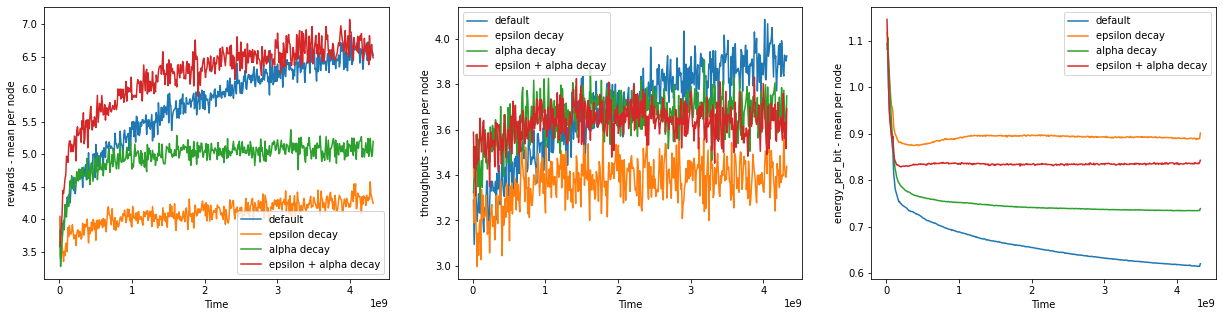
\includegraphics[scale=0.40]{plots/decays/tabular_q_learning_decay_SMALL.png}
  \caption{Q learning with alpha and epsilon decay}
\end{figure}

Here's a plot of effects of alpha and epsilon decay on tabular SARSA. As we can see from the rewards plot introducing alpha decay alone gives us the best result. This makes sense since learning rate adjustment is crucial for SARSA as 
\begin{figure}[H]
\centering
\hspace*{-3.3cm}  
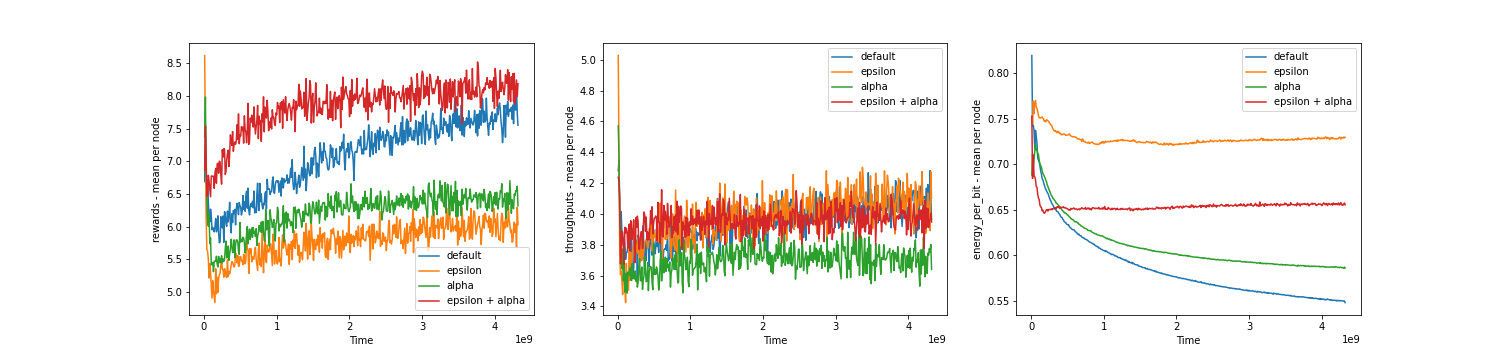
\includegraphics[scale=0.40]{plots/decays/decay_tabular_sarsa_SMALL.png}
  \caption{SARSA with alpha and epsilon decay}
\end{figure}

As can be seen for both deep q learning and sarsa benefit from
both epsilon and alpha decay. 

\begin{figure}[H]
\centering
\hspace*{-1.1cm}  
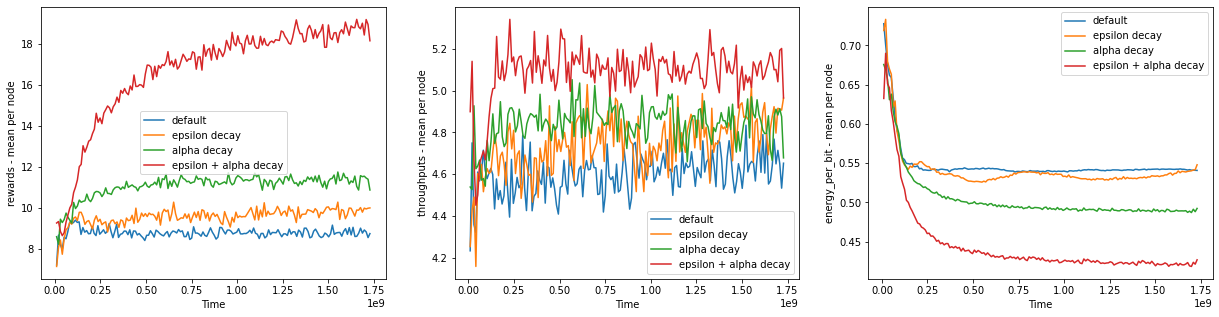
\includegraphics[scale=0.40]{plots/decays/deep_q_decay_SMALL.png}
  \caption{Deep Q learning with alpha and epsilon decay}
\end{figure}

\begin{figure}[H]
\centering
\hspace*{-1.1cm}  
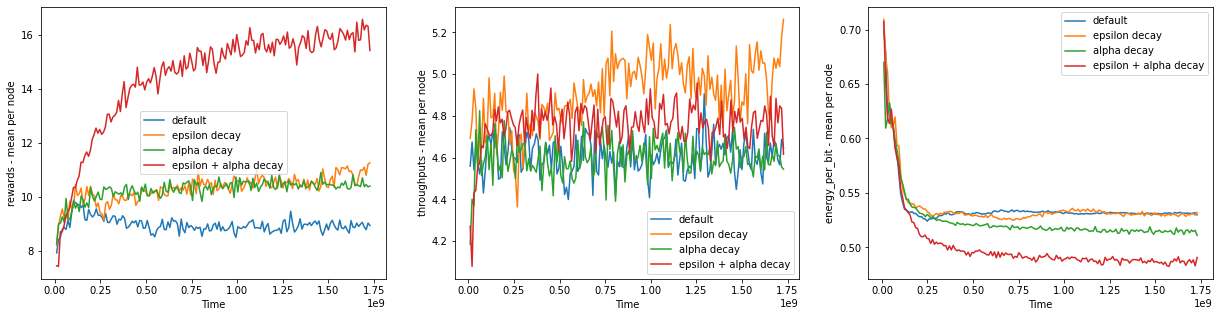
\includegraphics[scale=0.40]{plots/decays/deep_sarsa_decay_SMALL.png}
  \caption{Deep SARSA with alpha and epsilon decay}
\end{figure}

Here you can see all different flavours 
compared against each other. Each one 
has epslion and alpha decay enabled in the 
same way. We can see that as expected deep models outperform their tabular counterparts and Q-learning in particular outperforms SARSA.

\begin{figure}[H]
\centering
\hspace*{-3.3cm}  
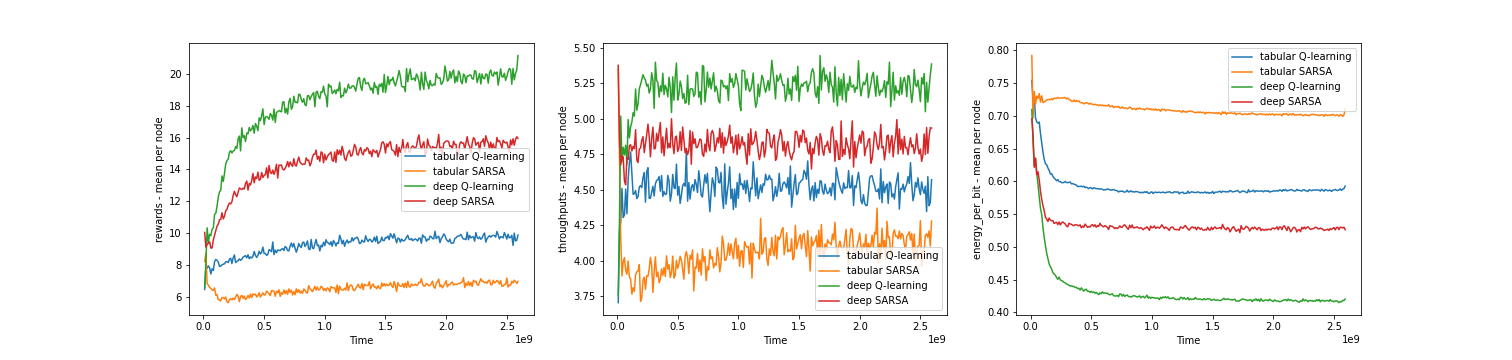
\includegraphics[scale=0.40]{plots/decays/all_decay_SMALL.png}
  \caption{All implementations}
\end{figure}

\subsection{Decay rate}

For all of the above a decay rate of 1 was used. What
that means is that for both epsilon and alpha the decay 
update happened every n steps, where n is the size of 
a cluster, that the agent is assigned to. This makes 
sense since ideally we would want a situation where
all nodes got involved with $\epsilon$ and $\alpha$
once before they got updated. Here are plots for both where i tried different decay rates. As it turns out for alpha in particular a rate of 0.5 produces better results than the default 
one.

\begin{figure}[H]
\centering
\hspace*{-3.3cm}  
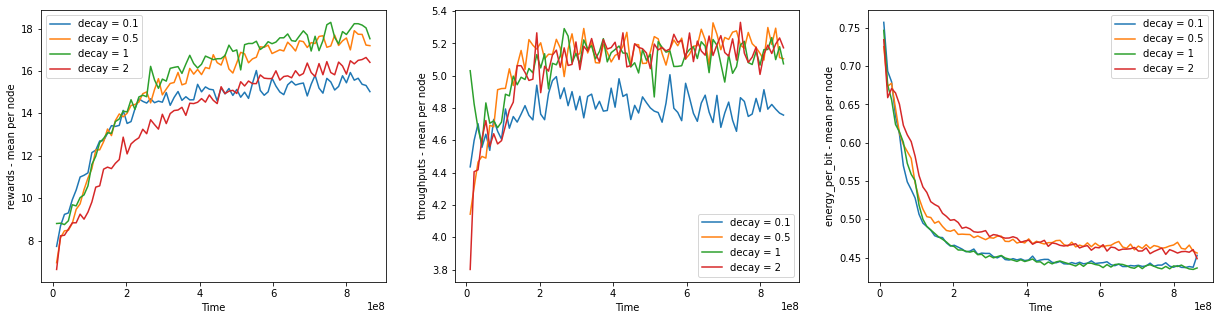
\includegraphics[scale=0.40]{plots/decays/epsilon_deep_q_SMALL.png}
  \caption{Epsilon decay rate}
\end{figure}

\begin{figure}[H]
\centering
\hspace*{-3.3cm}  
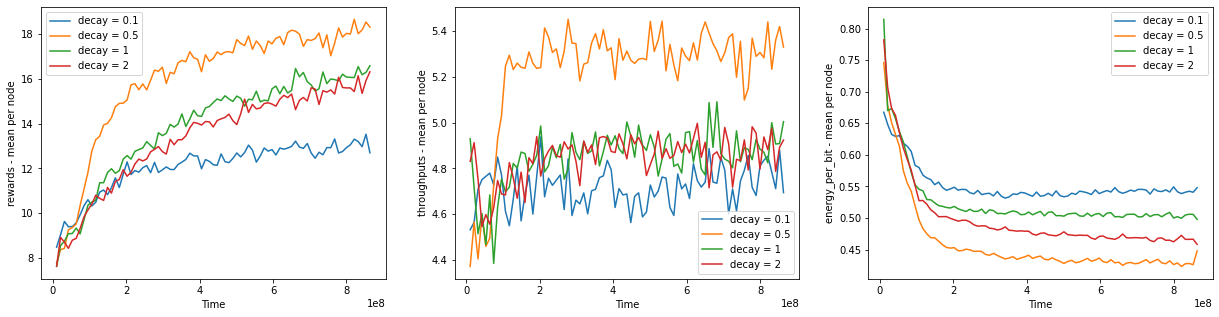
\includegraphics[scale=0.40]{plots/decays/alpha_deep_q_SMALL.png}
  \caption{Alpha decay rate}
\end{figure}

\section{Gamma}
here's a straightforward progression for gamma 
(discount factor) values. As we can see the model
learns best when we put more weight on future
decisions.

\begin{figure}[H]
\centering
\hspace*{-3.3cm}  
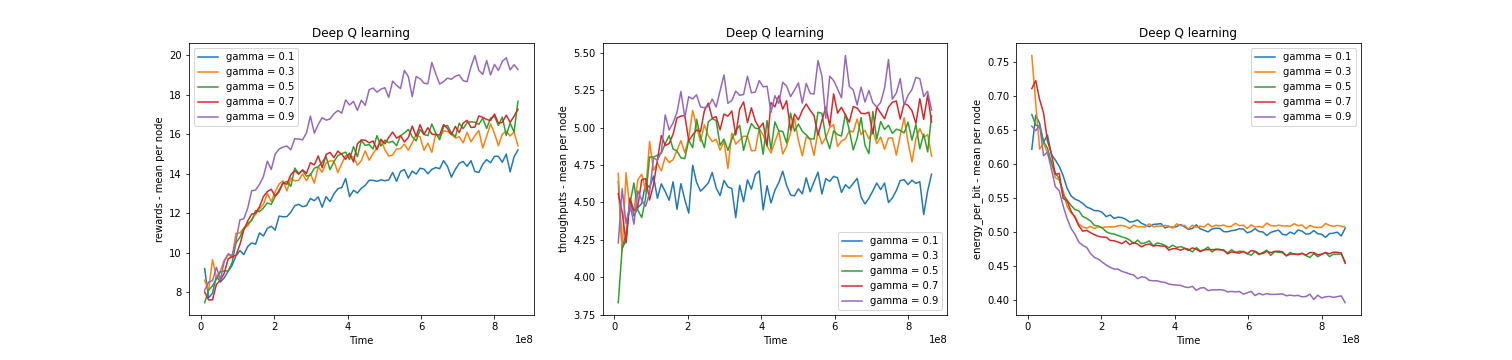
\includegraphics[scale=0.40]{plots/gamma/gamma_deep_q_SMALL.png}
  \caption{Tuning gamma}
\end{figure}


\section{State Space}
From the plots it is apparent that including 
\texttt{energy} dimension into the state space results in worse learning but that might also be due to the implementation in the simulation of information 
gathering.

Here is the comparison for fast action traversal. As we can see best options would
be \texttt{[tp]} and \texttt{[tp, sf, channel, sinr]} as they
produce similar rewards with former having 
better throughput while the latter has more optimal energy usage. 

\begin{figure}[H]
\centering
\hspace*{-3.3cm}  
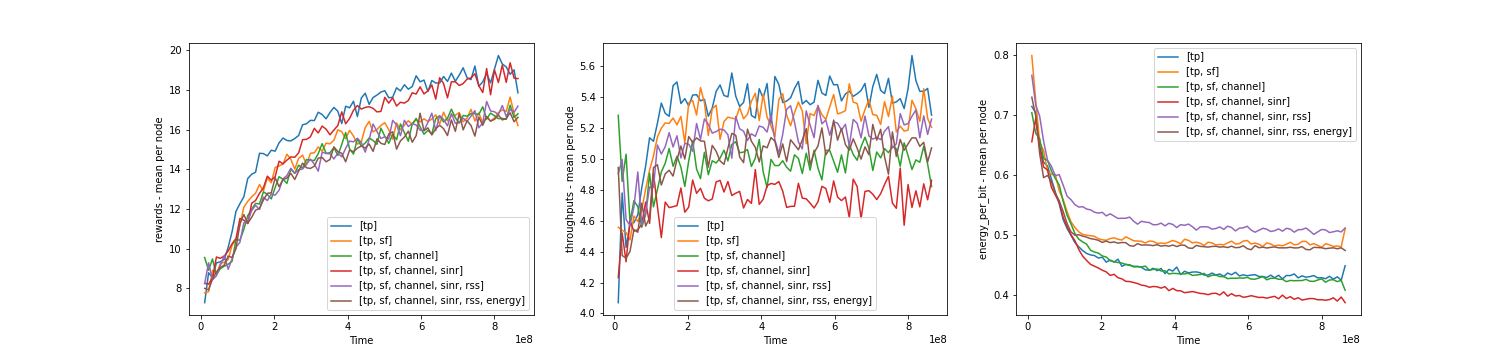
\includegraphics[scale=0.40]{plots/state_space/state_space_hypertuning_deep_q_SMALL.png}
  \caption{Tuning state space}
\end{figure}

Here's one for slow action. As we can see \texttt{[tp, sf]} and
\texttt{[tp, sf, channel]} are winning in this case.

\begin{figure}[H]
\centering
\hspace*{-3.3cm}  
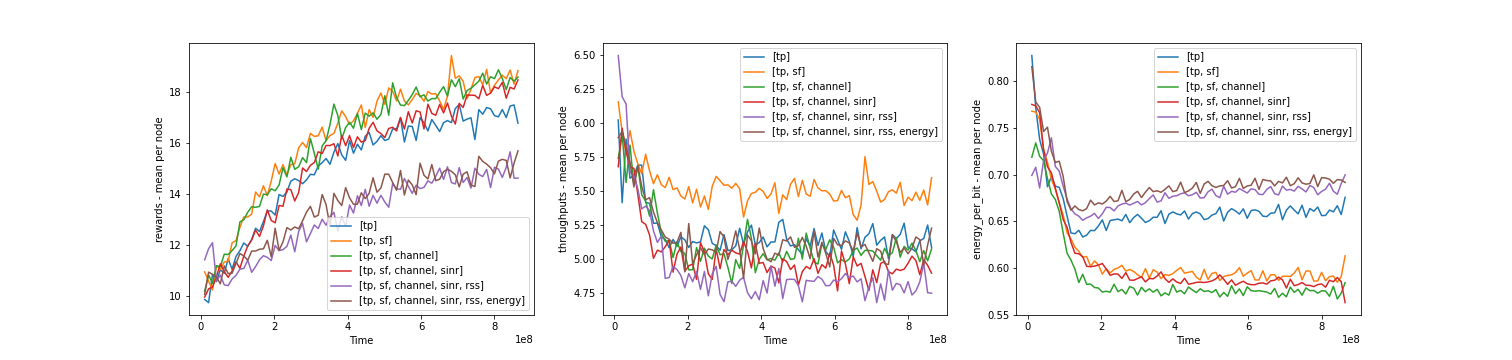
\includegraphics[scale=0.40]{plots/state_space/state_space_slow_action_hypertuning_deep_q_SMALL.png}
  \caption{Tuning state space}
\end{figure}

\section{Reward Function}

I have tried putting different emphasis on either 
throughput or energy via altering the basic reward formula of $\frac{throughput}{energy}$. \\

I have tried raising either numerator or denominator 
to powers of 2 and 3 to see if this will cause learning
to favour one more. The plots seem to suggest no apparent
effect (that is prior to convergence). 

\section{Slow Action Traversal}

As described above slow action traversal is possible in 
this scenario. Here are the plots comparing various
slow action traversal combinations.

\begin{figure}[H]
\centering
\hspace*{-3.3cm}  
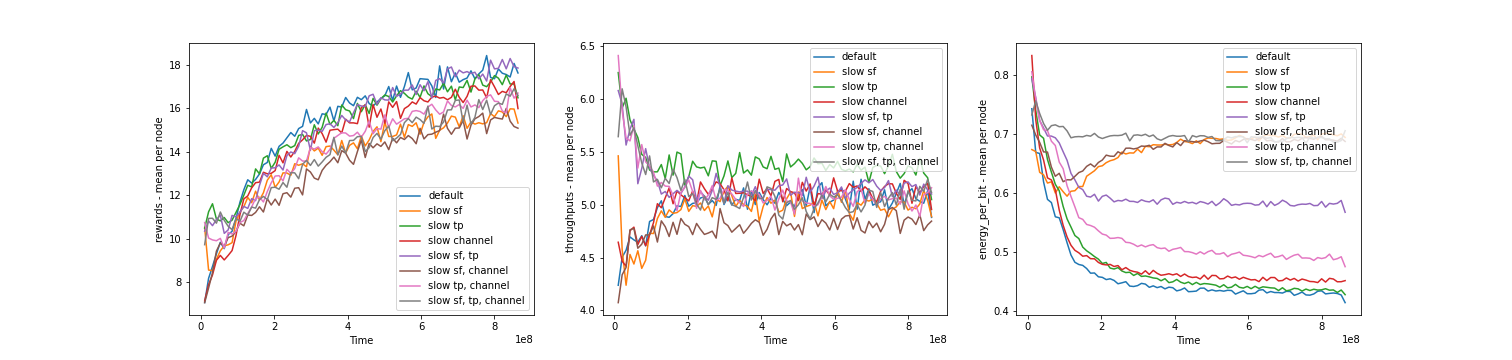
\includegraphics[scale=0.40]{plots/slow_action/slow_action_hypertuning_deep_q_SMALL.png}
  \caption{Slow action traversal}
\end{figure}

 No apparent
improvement can be seen from the default «fast»
action traversal, but we do notice that slowly 
traversing \texttt{tp} seems to improve throughput.
At the same time having only \texttt{[tp]} as a state space performed best for fast action traversal, so if we combine them we get: 

\begin{figure}[H]
\centering
\hspace*{-3.3cm}  
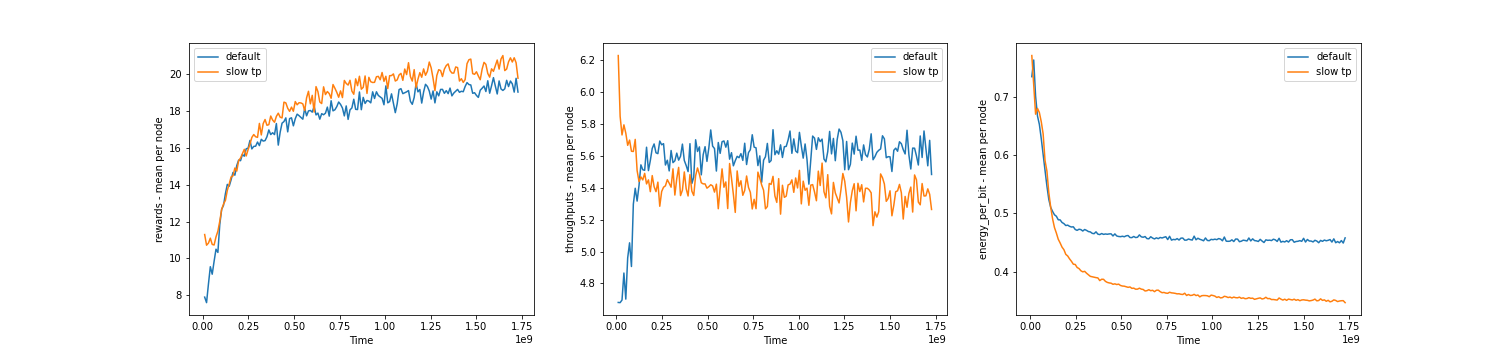
\includegraphics[scale=0.40]{plots/slow_action/slow_action__state_space_tp_hypertuning_deep_q_SMALL.png}
  \caption{Slow action traversal for \texttt{tp}}
\end{figure}

As we can see given a state space \texttt{[tp]} 
having slow \texttt{tp} action traversal improves
model performance.

% \subsection{Rates of update}
% These can be updated at each step, i.e. every time a node
% queries an agent or every now and then resulting in a 
% slower decay. As we see from the graphs slowing down the
% decay rate for both $\epsilon$ and $\alpha$ naturally
% results in a slower convergence but ends up higher 
% and gives better rewards in the end.\\

% Slowing down epsilon decay doesn't seem to have much effect
% on the throughput but improves energy usage.\\

% Slowing down alpha decay improves both energy and 
% throughput and results in a reward jump as well. 


\section{Tabular vs. Deep}
\section{SARSA vs Q-learning}
\section{Neural Network Depth}
\section{Prioritised Experience Replay Buffer}

Here's the plot for fast decay for epsilon and alpha along with slow action comparison.

\begin{figure}[H]
\centering
\hspace*{-3.3cm}  
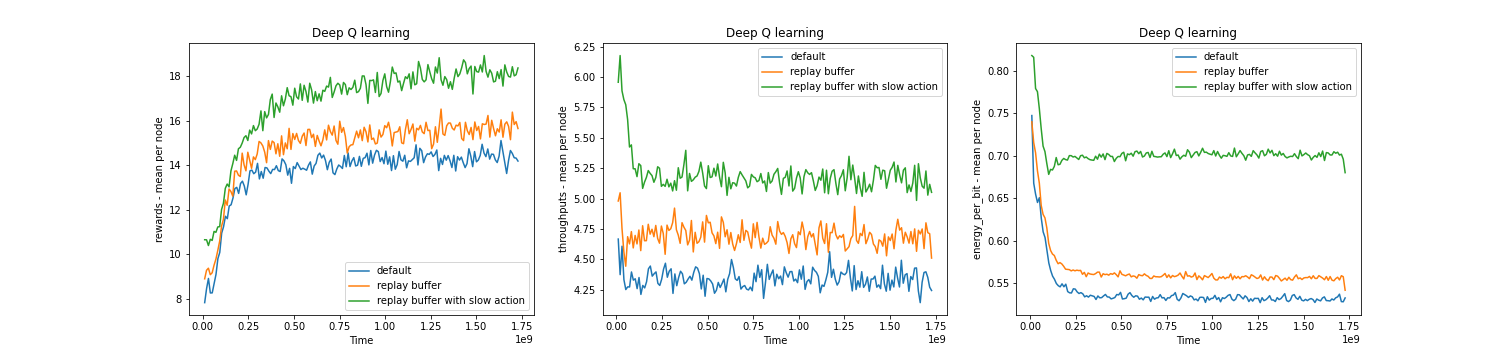
\includegraphics[scale=0.40]{plots/replay_buffer/replay_buffer_with_slow_action_traversal_fast_decay_deep_q_SMALL.png}
  \caption{buffer with fast decay}
\end{figure}

Here's the plot for slow decay for epsilon and alpha along with slow action comparison.

\begin{figure}[H]
\centering
\hspace*{-3.3cm}  
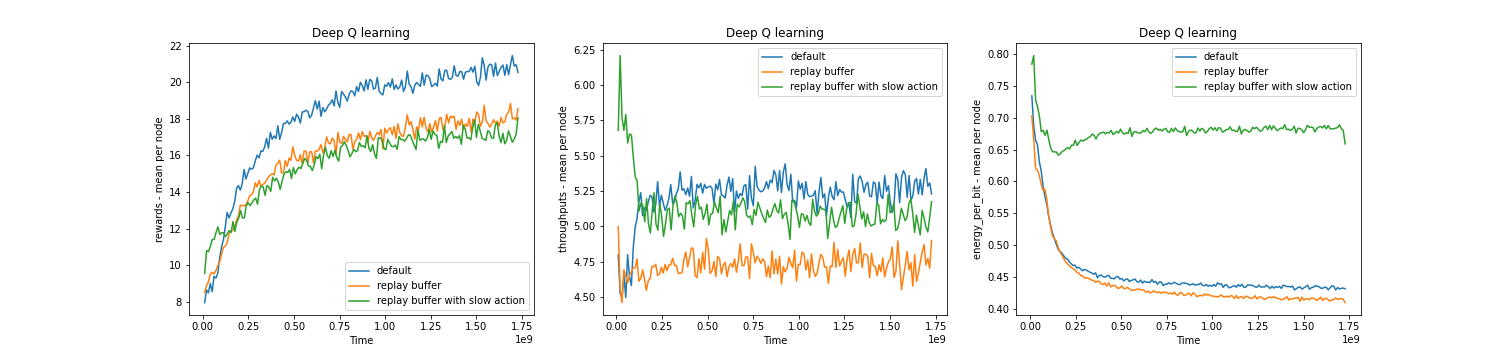
\includegraphics[scale=0.40]{plots/replay_buffer/replay_buffer_with_slow_action_traversal_deep_q_SMALL.png}
  \caption{buffer with slow decay}
\end{figure}

As we can see with fast decay replay buffer does benefit Q-learning substantially especially with the addition of slow action traversal, but if we slow down the decay rate for epsilon and alpha it actually worsens 
the default Deep Q-learning performance which still
performs better than the most optimal one 
if fast decay rates.

\subsection{Buffer size}
Here I conducted hypertuning on the buffer size.
For each run the buffer size is scaled by the 
respective number based on the cluster size, i.e.
if the agent is assigned to 8 nodes, with scaling
factor 3, buffer size is 24. 

\begin{figure}[H]
\centering
\hspace*{-3.3cm}  
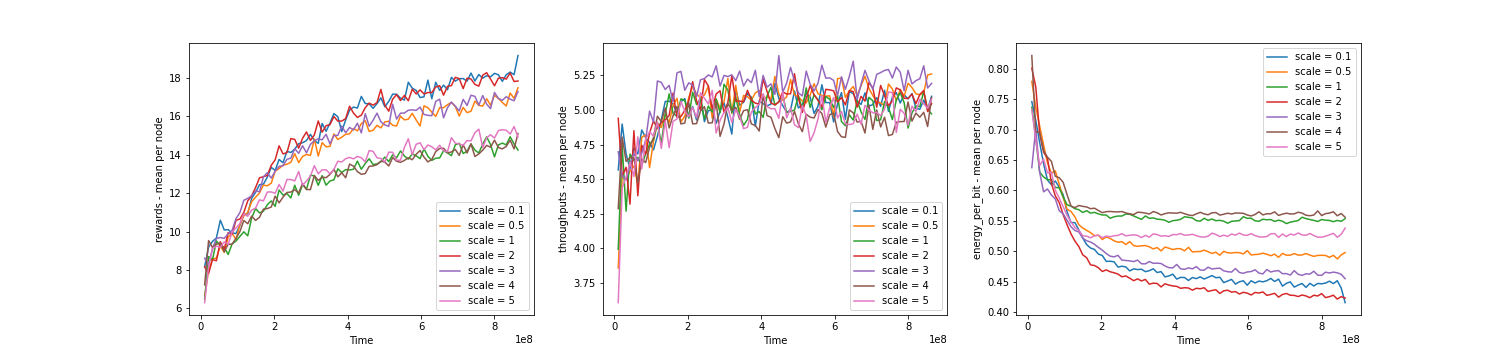
\includegraphics[scale=0.40]{plots/replay_buffer/replay_buffer_scale_deep_q_SMALL.png}
  \caption{Scaling replay buffer size}
\end{figure}

\section{Target Network and Double Deep learning}

Here's a plot trying out differernt update rates
for the target network as can be seen 2 is the optimal setting. That means target network is 
updated every \texttt{cluster\_size * 2} steps.

\begin{figure}[H]
\centering
\hspace*{-3.3cm}  
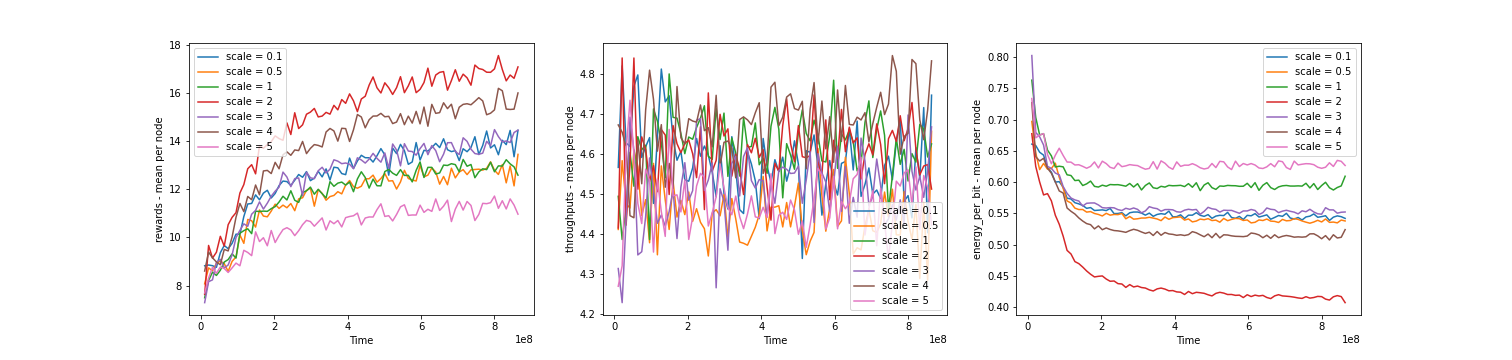
\includegraphics[scale=0.40]{plots/target_double_deep/target_update_rate_deep_q_SMALL.png}
  \caption{Scaling target network update rate}
\end{figure}

As can be seen based on the rewards and energy plots scale 2 is preferred.

\section{Comparison against default}

As we can see adding double deep learning along with
replay buffer does not benefit the learning and default
Q-learning still performs better (that is with decay
rate of one).

\begin{figure}[H]
\centering
\hspace*{-3.3cm}  
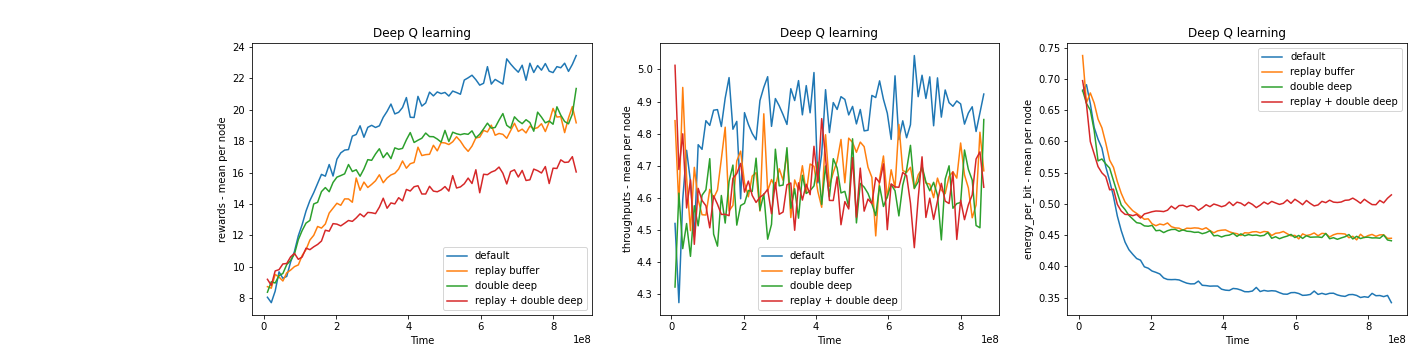
\includegraphics[scale=0.40]{plots/target_double_deep/replay_double_SMALL.png}
  \caption{Effect of introducing replay buffer and double deep learning}
\end{figure}

\section{Sector size}
As the plots show reducing sector size improves energy
usage and produces better reward curve. This makes sense,
since naturally each learning agent covers a smaller 
more specialized area of less nodes.
% \chapter{Evaluation}
% \section{ADR}
% \section{Comparing against other implementations}